% !TEX root = ../thesis.tex
% ==============================================================================
%  CHAPTER 4: PROPOSED METHODOLOGY (فصل چهارم: روش‌شناسی پیشنهادی) (chapters/chapter4_methodology.tex)
% ==============================================================================
%  This chapter details the theoretical formulation, architectural design,
%  and algorithmic pipeline of the proposed framework.
% ==============================================================================

\chapter{چارچوب پیشنهادی}\label{chap:chapter4_methodology}

این فصل، پایه‌ی فنی و روش‌شناختی این پایان‌نامه را بنا می‌نهد و به تشریح چارچوب پیشنهادی «جانشین مبتنی بر انرژی برای تفسیر در سطح مفهوم» (\lr{ESCI}) می‌پردازد. با توجه به چالش‌های بنیادین مطرح‌شده در فصل‌های پیشین، این چارچوب با هدف غلبه بر انسداد مدل‌های جعبه‌سیاه و رفع نارسایی‌های روش‌های تفسیرپذیری توکن‌محور طراحی شده است. در این فصل، ابتدا معماری پیش‌پردازش و استخراج ویژگی‌ها تبیین می‌گردد، سپس جزئیات ریاضی و ساختاری فازها به‌دقت فرمول‌بندی شده و در نهایت، الگوریتم آموزش مشترک و بهینه‌سازی تناوبی این سیستم دوفازی ارائه می‌شود.



\section{نمای کلی و فرمول‌بندی مسئله}\label{sec:4-1}

همان‌گونه که در فصل‌های پیشین (به‌ویژه بخش‌های~\ref{sec:2-3-3} و~\ref{sec:3-1-3-2}) واکاوی شد، تقلیل‌گرایی توکن‌محور و اعمال اختلالات خرد در ممیزی مدل‌های جعبه‌سیاه، ناگزیر به تخریب ساختار نحوی، بروز خطای شوک توزیعی و کوری معنایی می‌انجامد. برای گریز از این بن‌بست، رویکردهایی نظیر یکپارچه‌سازی ویژگی‌های خام به مفاهیم کلان (مانند تقطیع پیکسل‌ها به اشیاء فیزیکی در پردازش تصویر~\cite{cafagna2023interpreting}) پیشنهاد شده‌اند. با این حال، انتقال این راهبرد به زبان طبیعی با یک مانع ساختاری مواجه است؛ چرا که تحدید مرزهای یک مفهوم انتزاعی در متن به‌سادگی مرزبندی اشیاء در تصویر نیست. در پاسخ به این شکاف، چارچوب پیشنهادی این پژوهش (\lr{ESCI})، با الگوبرداری از ایده‌ی تجمیع پیش‌فرض‌های معنایی اما متناسب با ذات زبان، واحد تحلیل را از سطح توکن به جمله ارتقا می‌دهد. با اتکا به اصل بافتار فرگه~\cite{frege1991foundations} و مدل شناختی ساخت‌وساز-ادغام کینتش~\cite{kintsch1998comprehension}، روشن گردید که نشانه‌های گسسته در انزوا فاقد استقلال معنایی‌اند و هویت گزاره‌ای در افق جملات کامل پدیدار می‌شود. در این راستا و همگام با سایر روش‌های مبتنی بر جمله به‌عنوان واحد پردازش~\cite{lcmteam2024lcm, enouen2024textgenshap, wang2023prompting}، با اتخاذ جمله به‌عنوان یک مفهوم عملیاتی با مرزهای نحوی مشخص، چارچوب \lr{ESCI} به‌گونه‌ای پیکربندی شده است که وابستگی‌های گزاره‌ای و میزان تأثیر هر بخش از پرامپت ورودی را بر خروجی هدف، بدون بروز گسست نحوی و شوک توزیعی ردیابی نماید.

مسئله‌ی اصلی این پایان‌نامه، تفسیر رفتار یک مدل زبانی جعبه‌سیاه از طریق انتخاب ویژگی در سطح نمونه است. مطابق با مبانی صوری پایه‌ریزی‌شده در بخش~\ref{sec:1-1-1}، مدل زبانی بزرگ به‌صورت یک نگاشت مولد جعبه‌سیاه $f_\theta: \mathcal{S}^N \to \mathcal{S}^M$ در نظر گرفته می‌شود که تنها از طریق استعلام‌های مرتبه‌صفر در دسترس است و در پاسخ به پرامپت ورودی $\mathbf{x}$، متن خروجی $\mathbf{y} = f_\theta(\mathbf{x})$ را تولید می‌کند. بر پایه‌ی تعریف~\ref{def:chap1_proposition_space}، پرامپت خام کاربر از طریق عملگر تقطیع نحوی $\Pi$ به دنباله‌ای از $N$ جمله (گزاره) افراز می‌گردد (معادله‌ی~\ref{eq:chap1_prompt_decomp}):
\begin{equation}\label{eq:chap4_prompt_def}
    \mathbf{x} = (x_1, x_2, \dots, x_N) \in \mathcal{S}^N
\end{equation}
به‌طور مشابه، پاسخ محقق‌شده توسط مدل زبانی جعبه‌سیاه نیز به دنباله‌ای از $M$ جمله تجزیه می‌شود (معادله‌ی~\ref{eq:chap1_response_decomp}):
\begin{equation}\label{eq:chap4_response_def}
    \mathbf{y} = (y_1, y_2, \dots, y_M) \in \mathcal{S}^M
\end{equation}
در این سناریوی انتساب، تحلیل‌گر زیرمجموعه‌ای مشخص از شاخص‌های جملات خروجی مورد نظر با عنوان $T \subseteq \{1, 2, \dots, M\}$ با کاردینالیتی $|T| = M_T \le M$ را به‌عنوان شاخص‌های هدف تعیین می‌کند که توالی جملات هدف خروجی را به‌صورت $\mathbf{y}_T = {(y_j)}_{j \in T} \subseteq \mathbf{y}$ بر مبنای تعریف~\ref{def:chap1_target_subset} شکل می‌دهد:
\begin{equation}\label{eq:chap4_target_def}
    \mathbf{y}_T = {(y_j)}_{j \in T} \subseteq \mathbf{y}
\end{equation}
که در حالت ارزیابی یک گزاره‌ی منفرد، $T = \{t\}$ و $\mathbf{y}_T = y_t$ خواهد بود.

بر اساس تعریف~\ref{def:chap1_mask_space}، هدف از انتساب در سطح جمله، شناسایی زیرمجموعه‌ای از جملات پرامپت ورودی به‌عنوان پیش‌آیندهای گزینش‌شده ($\mathbf{x}_S \subseteq \mathbf{x}$) است که بیشترین تأثیر را بر تولید گزاره‌های هدف خروجی $\mathbf{y}_T$ داشته‌اند. با تعریف فضای فرضیات انتساب بر روی مشبکه‌ی بولی $\mathcal{M} = {\{0, 1\}}^N$، هر بردار ماسک دودویی $\mathbf{m} = {(m_1, m_2, \dots, m_N)}^\top \in \mathcal{M}$ زیرمجموعه‌ی پیش‌آیند ورودی را با استفاده از عملگر ضرب هادامارد ($\odot$) استخراج می‌نماید:
\begin{equation}\label{eq:chap4_mask_def}
    \mathbf{x}_S = \mathbf{x} \odot \mathbf{m} = \{ x_i \in \mathbf{x} \mid m_i = 1, \, i \in \{1, \dots, N\} \}
\end{equation}
و زیرمجموعه‌ی متمم یا دورریز به‌صورت $\mathbf{x}_{\text{\lr{discard}}} = \mathbf{x} \odot (\mathbf{1} - \mathbf{m}) = \mathbf{x} \setminus \mathbf{x}_S$ به‌دست می‌آید. در این بردار ماسک، درایه‌ی $m_i = 1$ نشان می‌دهد که جمله‌ی ورودی $x_i$ به‌عنوان یک پیش‌آیند اثرگذار بر شکل‌گیری $\mathbf{y}_T$ شناسایی شده است و $m_i = 0$ نمایانگر عدم‌وابستگی گزاره‌ی هدف به آن جمله در ورودی است. همان‌گونه که در مسئله‌ی~\ref{prob:chap1_causal_attribution} در فصل اول صورت‌بندی شد، حل دقیق این مسئله مستلزم کمینه‌سازی هم‌زمان اندازه‌ی ماسک (اصل ضرورت و فشردگی) و تضمین بازتولید خروجی هدف توسط پیش‌آیندهای منتخب (اصل کفایت) است:
\begin{equation}\label{eq:chap4_constrained_opt}
    \mathbf{m}^* = \arg\min_{\mathbf{m} \in {\{0, 1\}}^N} \|\mathbf{m}\|_0 \quad \text{به‌شرط آنکه} \quad \mathcal{D}\big(f_\theta(\mathbf{x} \odot \mathbf{m}), \mathbf{y}_T\big) \le \epsilon
\end{equation}
که در آن $\mathcal{D}$ سنجه‌ی واگرایی معنایی در فضای خروجی مدل و $\epsilon > 0$ حد آستانه‌ی خطای پذیرفتنی است.

برای حل این مسئله‌ی بهینه‌سازی در یک محیط جعبه‌سیاه مسدود، و برای فرار از فراخوانی‌های نمایی رابط برنامه‌نویسی (\lr{API}) که در روش‌های اختلالی کلاسیک وجود دارد، ما از پارادایم آموزش سراسری یک مفسر محلی که در بخش~\ref{sec:3-1-3-3} شرح داده شد، بهره می‌بریم. برخلاف مفسرهای محلی کلاسیک (مانند \lr{LIME}) که تنها همسایگی‌های بلافصل را بررسی می‌کنند و اغلب منجر به توهم تفسیرپذیری می‌شوند، مدل ما روی توزیع گسترده‌تری آموزش می‌بیند تا الگوهای تولید سراسری را درک کند. نمای کلی این سیستم در شکل~\ref{fig:chap4_framework_overview} به تصویر کشیده شده است.

\begin{figure}[ht]
    \centering
    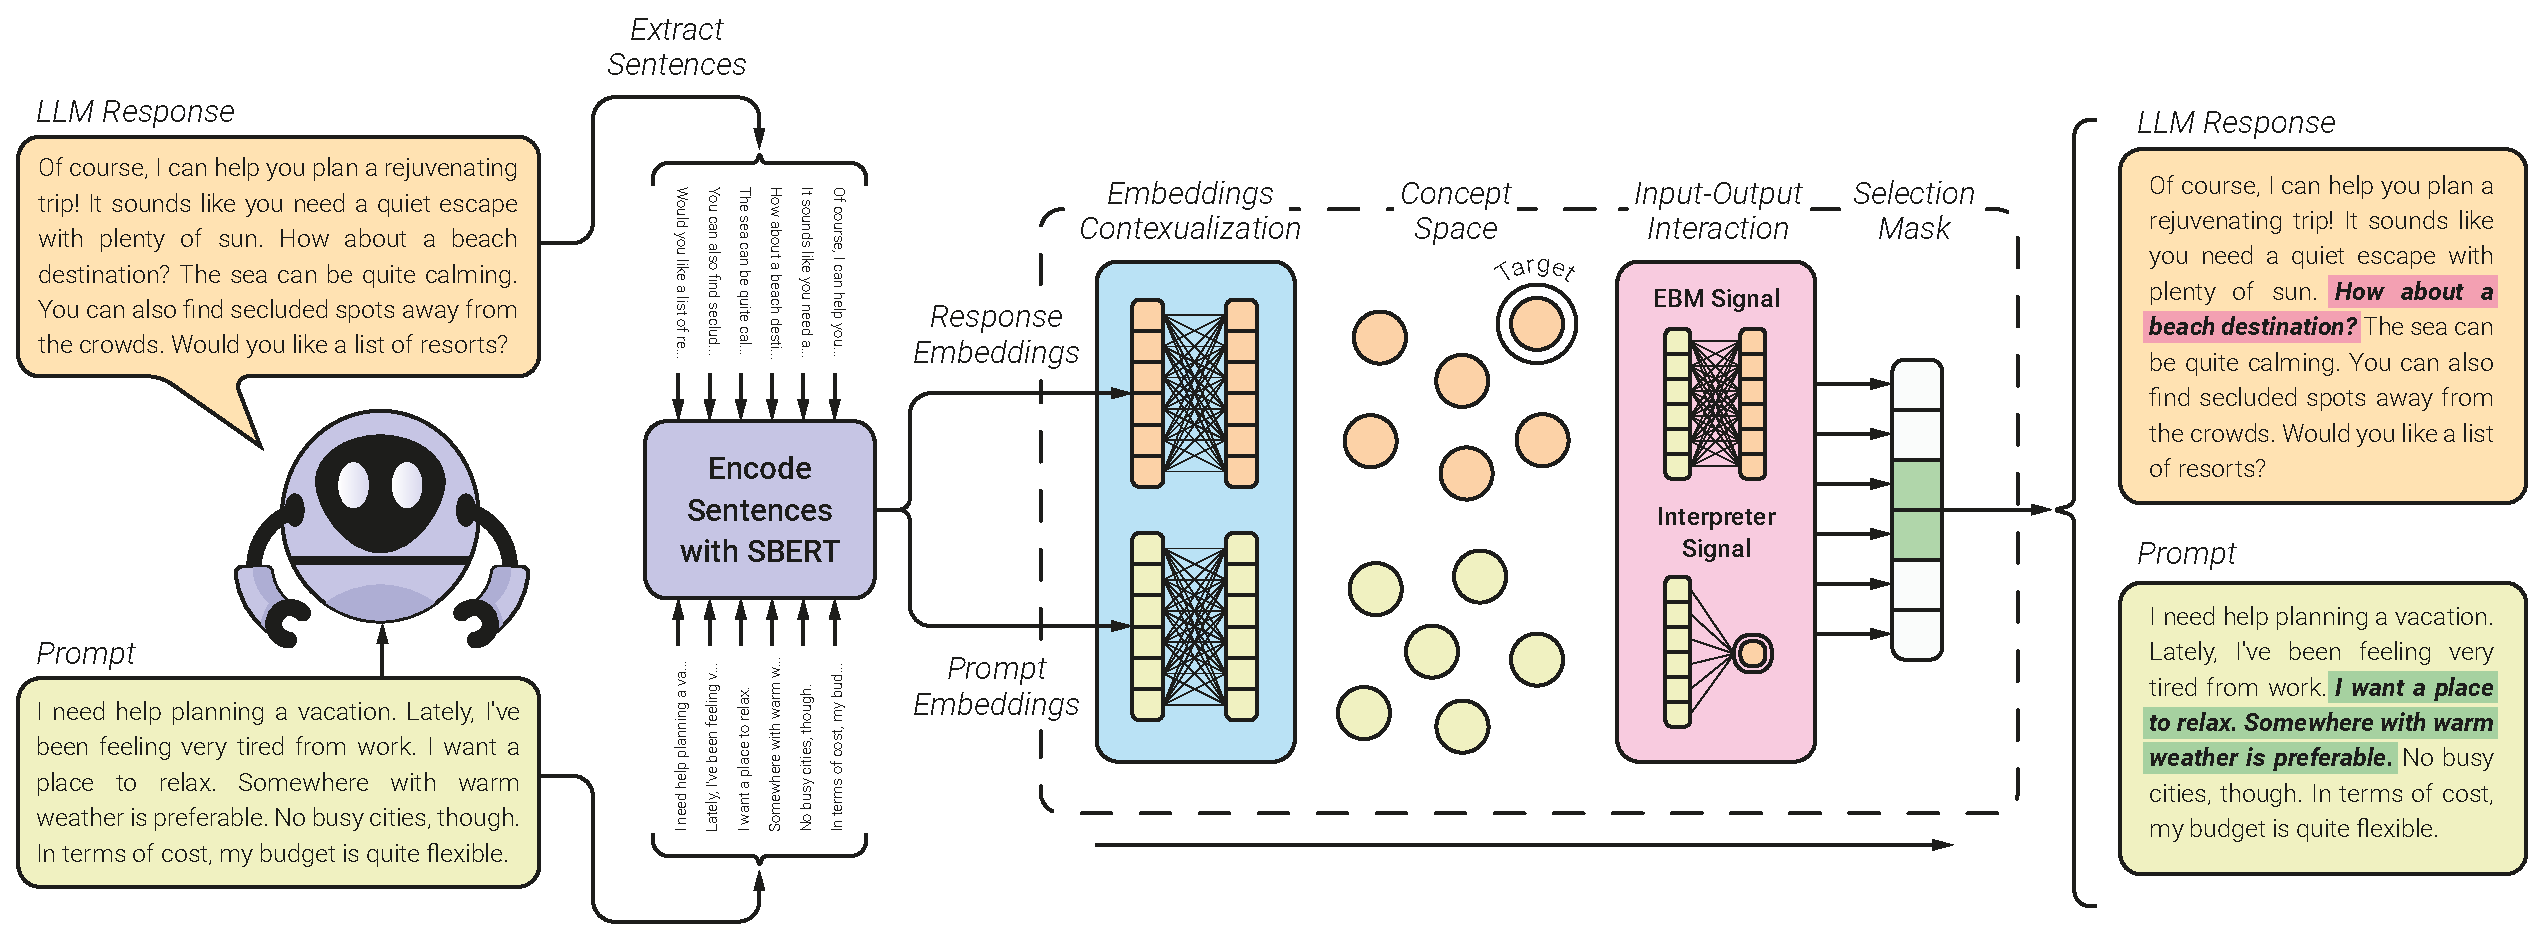
\includegraphics[width=\textwidth]{figures/Fig-Framework-Overview-V5.pdf}
    \caption{نمای کلی چارچوب پیشنهادی (\lr{ESCI})}\label{fig:chap4_framework_overview}
\end{figure}

همان‌طور که در شکل~\ref{fig:chap4_framework_overview} مشاهده می‌شود، روند اجرای این خط‌لوله از چپ به راست طی می‌شود. برای یک جفت (پرامپت، پاسخ) داده‌شده از مدل زبانی جعبه‌سیاه، ابتدا متن به جملات مجزا شکسته شده و توسط یک مدل پیش‌آموزش‌دیده مانند \lr{Sentence-BERT} به بردارهای تعبیه تبدیل می‌شود. سپس، ماژول‌های تصویرساز این تعبیه‌ها را زمینه‌سازی کرده و آن‌ها را به یک فضای مفهومی مشترک نگاشت می‌کنند؛ فضایی که در آن مجاورت هندسی بردارها نشان‌دهنده‌ی ارتباطات متنی جملات است. پس از تعیین شاخص‌های هدف خروجی ($T$)، ماژول تعاملی میزان انطباق‌پذیری ساختاری میان مفاهیم ورودی و خروجی را ارزیابی می‌کند. این ماژول‌ها با بهره‌گیری از سیگنال‌های دریافتی از یک شبکه‌ی انرژی که میزان انطباق‌پذیری ساختاری و معنایی میان ورودی و خروجی را بر اساس الگوهای متنی مدل هدف ارزیابی می‌کند، هدایت می‌شوند. شبکه‌ی مفسر با دریافت پرامپت کامل، خروجی کامل و شاخص‌های هدف خروجی، ماسک اهمیتی تولید می‌نماید که پیش‌آیندهای اثرگذار ورودی را برای گزاره‌های هدف خروجی مشخص می‌سازد. در نهایت، همان‌طور که در سمت راست تصویر نمایان است، با اعمال این ماسک، جملات پیش‌آیند منتخب ورودی استخراج می‌شوند.

شایان ذکر است که این شکل تنها یک نمای کلی از فرایند را نشان می‌دهد و فازهای مجزا را به‌تفکیک در بر ندارد. به‌منظور تحقق این فرایند، به‌جای جستجوی پرهزینه در فضای خروجی مدل هدف، معماری \lr{ESCI} بر اساس دو فاز درهم‌تنیده بنا شده است که در ادامه‌ی این فصل با جزئیات بررسی خواهند شد:

\begin{enumerate}
    \item \textbf{فاز اول (مدل جانشین مبتنی بر انرژی):} در این فاز، یک مدل مبتنی بر انرژی (\lr{EBM}) با معماری ترنسفورمر دوسویه ($\mathcal{E}_{\text{\lr{LM}}}(\mathbf{x}, \mathbf{y}; \theta)$) به‌عنوان مدل جانشین آموزش می‌بیند تا میزان انطباق‌پذیری ساختاری و معنایی میان پرامپت ورودی و پاسخ تولیدشده را بر مبنای الگوهای متنیِ مشاهده‌پذیر ارزیابی کند. دلیل انتخاب \lr{EBM} این است که فرایند انتساب نیازمند ارزیابی انطباق‌پذیری در سطح توالی کامل است؛ ساختاری که بدون وابستگی به نرمال‌سازی محاسبه‌ناپذیر احتمالات روی فضای نمایی خروجی‌ها و بدون نیاز به لوجیت‌ها یا فعال‌سازی‌های درونی، میزان همخوانی پرامپت و پاسخ را در قالب یک تابع انطباق‌پذیریِ نرمال‌نشده ارزیابی می‌نماید. این شبکه یک تابع انرژی اسکالر می‌آموزد که سطوح پایین‌تر آن بازتاب‌دهنده‌ی انطباق‌پذیری بالاتر بر اساس مشاهدات متنی است.
    
    \item \textbf{فاز دوم (شبکه‌ی مفسر هدایت‌شده):} در فاز عملیاتی، یک شبکه‌ی مفسر مستقل ($\mathcal{IN}(\mathbf{x}, \mathbf{y}, T; \alpha)$) با معماری ترنسفورمر دوسویه، برای تولید بردار ماسک اهمیت ($\mathbf{m}$) طراحی شده است. این مفسر پرامپت کامل ($\mathbf{x}$)، پاسخ کامل تولیدشده ($\mathbf{y}$) و مجموعه‌ی شاخص‌های هدف خروجی ($T$) را دریافت کرده و با شرطی‌سازی بازنمایی‌های خروجی بر روی شاخص‌های هدف و بهره‌گیری از سیگنال‌های دریافتی از چشم‌انداز انرژی مدل جانشین، یاد می‌گیرد که اثرگذارترین پیش‌آیندهای پرامپت را شناسایی و استخراج نماید. پس از اتمام آموزش، شبکه‌ی مفسر به‌صورت مستقل و در زمان‌ثابت برای انتساب نمونه‌های جدید به‌کار گرفته می‌شود.
\end{enumerate}

طراحی این رویکرد دوفازی مفسر را قادر می‌سازد تا تنها با یک بار عبور پیش‌رو در گراف محاسباتی خود و بدون نیاز به استعلام مجدد از مدل جعبه‌سیاه در زمان استنتاج، پیش‌آیندهای اثرگذار را استخراج نماید. در بخش‌های بعدی، مراحل پیش‌پردازش، معماری دقیق لایه‌ها و الگوریتم‌های بهینه‌سازی توأم در هر یک از این دو فاز به‌تفصیل فرمول‌بندی خواهند شد.



\section{پیش‌پردازش و استخراج ویژگی‌ها}\label{sec:4-2}

پردازش متون طبیعی توسط معماری‌های عصبی پیشرفته، نیازمند گذار از فضای نمادین و گسسته‌ی کلمات به یک فضای برداری پیوسته و محاسبه‌پذیر است. از آنجا که چارچوب پیشنهادی ما (\lr{ESCI}) واحد تحلیل خود را بر مبنای مفاهیم گزاره‌ای (جملات) استوار کرده است، خط‌لوله‌ی ورود داده‌ها به مدل باید به‌گونه‌ای طراحی شود که علاوه بر استخراج دقیق این واحدهای معنایی، آن‌ها را در قالب ماتریس‌هایی با ابعاد ثابت و منطبق با مکانیزم‌های توجهِ ترنسفورمرها آماده‌سازی کند.

این فرایند در سه گام اساسی تقطیع، تعبیه‌سازی، و نرمال‌سازی ابعاد انجام می‌پذیرد.


\subsection{تقطیع جملات}\label{sec:4-2-1}

نخستین گام در آماده‌سازی داده‌ها، شکستن متن خام ورودی (پرامپت کاربر) و خروجی (پاسخ مدل زبانی) به دنباله‌ای از گزاره‌ها یا به‌طور دقیق‌تر جملات است. برای انجام این تقطیع، از کتابخانه‌ی پردازش زبان طبیعی \lr{spaCy}~\cite{honnibal2017spacy} استفاده می‌شود. این ابزار که توسط شرکت \lr{Explosion AI} توسعه یافته است، یک کتابخانه‌ی متن‌باز و صنعتی است که برخلاف ابزارهای سنتی‌تر (مانند \lr{NLTK}~\cite{loper2002nltk} که بیشتر با اهداف آموزشی و مبتنی بر روش‌های آماری ساده‌تر طراحی شده‌اند)، مشخصاً برای پیاده‌سازی‌های سریع و کاربردهای عملیاتی در مقیاس بزرگ بهینه‌سازی شده است.

مزیت اصلی \lr{spaCy} در تقطیع جملات، اتکای آن به تجزیه‌گر وابستگی نحوی است. در حالی که روش‌های کلاسیک اغلب به علائم نگارشی (مانند نقطه یا علامت سؤال) یا عبارات منظم\enfootnote{regex} وابسته‌اند و در مواجهه با متن‌های بدون ساختار، اختصارات، یا خروجی‌های نامنظم مدل‌های زبانی دچار خطای مرزبندی می‌شوند، \lr{spaCy} با ساخت یک درخت نحوی از کلمات، مرز جملات را بر اساس ساختار دستوری و روابط وابستگی میان توکن‌ها شناسایی می‌کند. این رویکرد به سیستم اجازه می‌دهد تا حتی در متون پیچیده و فاقد علائم نگارشی استاندارد نیز با دقت بالایی عمل کند.

با اعمال این تقطیع، پرامپت خام $\mathbf{x}$ به دنباله‌ای از $N$ جمله‌ی مجزا ($x_1, x_2, \dots, x_N$) و پاسخ خام $\mathbf{y}$ به دنباله‌ای از $M$ جمله‌ی مجزا ($y_1, y_2, \dots, y_M$) تبدیل می‌شوند. این عملیات تضمین می‌کند که بلوک‌های سازنده‌ی تحلیل ما، قطعات تکه‌تکه‌شده‌ی گرامری نبوده و واحدهایی حامل یک فکر یا ایده‌ی کامل باشند که از منظر منطقی و معنایی قابل‌ارزیابی‌اند.


\subsection{تولید تعبیه‌ها}\label{sec:4-2-2}

پس از استخراج جملات، هر جمله‌ی گسسته باید به یک بردار متراکم در فضایی پیوسته نگاشت شود تا ماشین قادر به درک ویژگی‌های معنایی آن باشد. برای تحقق این امر، از ماژول پیش‌آموزش‌دیده‌ی \lr{Sentence-BERT}~\cite{reimers2019sentencebert} استفاده می‌کنیم. همان‌گونه که در بخش~\ref{sec:2-3-4} تشریح شد، این معماری سیامی آموزش دیده است تا جملاتی را که از نظر معنایی مشابه‌اند، به بردارهایی با فاصله‌ی هندسی نزدیک به هم نگاشت کند. لازم به ذکر است که این نزدیکی صرفاً سطحی بوده و مدل برای تولید تعبیه‌های جملات به‌صورت مستقل عمل می‌کند؛ لذا تعبیه‌های حاصل از این مرحله، میان جملات مستقل هستند و اطلاعاتی از هم برای درک بهتر بستر کل متن ندارند. به‌عبارتی، می‌توان گفت تعبیه‌های حاصل برای هر جمله مانند تعبیه‌های حاصل برای هر توکن در خط‌لوله‌ی ترنسفورمر پیش از ورود به معماری اصلی هستند.

در اجرای این چارچوب (برای مثال با بهره‌گیری از مدل \texttt{all-mpnet-base-v2}~\cite{song2020mpnet})، وزن‌های شبکه‌ی تعبیه‌ساز به‌طور کامل منجمد نگه‌داشته می‌شوند تا ویژگی‌های معنایی ایستا و ارگانیک جملات بدون دست‌خوردگی حفظ شوند. با عبور جملات پرامپت و پاسخ از این ماژول، هر جمله به یک بردار پیوسته با طول $d$ نگاشت می‌گردد. در نتیجه، رشته‌ی جملات پرامپت به یک دنباله از بردارهای تعبیه $S^{\text{\lr{in}}}$ و جملات پاسخ به دنباله‌ای از تعبیه‌های $S^{\text{\lr{out}}}$ تبدیل می‌شوند:
\begin{align}
    S^{\text{\lr{in}}} &= (\mathbf{e}_{x_1}, \mathbf{e}_{x_2}, \dots, \mathbf{e}_{x_N}) \label{eq:chap4_embed_in} \\
    S^{\text{\lr{out}}} &= (\mathbf{e}_{y_1}, \mathbf{e}_{y_2}, \dots, \mathbf{e}_{y_M}) \label{eq:chap4_embed_out}
\end{align}
که در آن هر $\mathbf{e}_i \in \mathbb{R}^d$ نشان‌دهنده‌ی بردار تعبیه‌ی یک جمله است و $d$ (که در پیاده‌سازی ما برابر با ۷۶۸ است) ابعاد فضای تعبیه‌ی \lr{Sentence-BERT} را مشخص می‌کند. این دنباله‌ها، نقشی مشابه با تعبیه‌ی توکن‌ها را برای معماری ترنسفورمری دوسویه‌ی ما ایفا می‌کنند، با این تفاوت که هر عضو دنباله، بار معنایی یک جمله‌ی کامل را در خود جای داده است.


\subsection{نرمال‌سازی و پدینگ}\label{sec:4-2-3}

شبکه‌های عصبی عمیق، به‌ویژه بلوک‌های مجهز به مکانیزم توجه با ابعاد ثابت، برای پردازش موازی دسته‌ای داده‌ها نیازمند دریافت ماتریس‌هایی با ابعاد کاملاً یکسان هستند. از آنجا که تعداد جملات در پرامپت‌ها ($N$) و پاسخ‌ها ($M$) در واقعیت همواره متغیر است، ما از یک استراتژی پدینگ اختصاصی بهره می‌بریم.

بدین‌منظور، یک ابرپارامتر وابسته به وظیفه تحت عنوان حداکثر طول دنباله یا $N_{\text{\lr{max}}}$ تعریف می‌شود. برای تعیین این ابرپارامتر، تحلیلی بر توزیع آماری تعداد جملات در وظیفه‌ی مورد نظر صورت گرفته و بنا به ملاحظات ساختاری، اندازه‌ی بیشینه‌ی مناسب تعیین می‌گردد. پس از تعیین این مقدار، عملیات نرمال‌سازی به رویه‌ی تشریح‌شده انجام می‌شود.

اگر تعداد جملات یک متن (مثلاً $N$) بیشتر از $N_{\text{\lr{max}}}$ باشد، دنباله تا رسیدن به این سقف مجاز بُرش می‌خورد و بخش‌های مازاد حذف می‌شوند. در مقابل، اگر متن کوتاه‌تر از $N_{\text{\lr{max}}}$ باشد، فضاهای خالی در انتهای دنباله با استفاده از تعبیه‌های قابل‌یادگیری به‌عنوان پدینگ پر می‌شوند. برخلاف پدینگ سنتی با بردار صفر، استفاده از بردارهای جای‌نگه‌دار با وزن‌های قابل‌یادگیری به مدل جانشین انرژی اجازه می‌دهد تا در فاز آموزش، رفتار مناسبی را برای نادیده گرفتن این بخش‌های خالی بیاموزد و محاسبات مکانیزم توجه را دچار سوگیری نکند. لازم به ذکر است که ماسک‌گذاری پدینگ نیز طبق اصول معماری ترنسفورمر در این معماری فعال بوده و پدینگ‌ها اثر مستقیم بر محاسبات ندارند.

با اعمال این مرحله‌ی نرمال‌سازی ابعادی، دنباله‌های متغیر ورودی به ماتریس‌هایی با ابعاد ثابت و پایدار تبدیل می‌شوند:
\begin{equation}\label{eq:chap4_final_tensors}
    S^{\text{\lr{in}}}, S^{\text{\lr{out}}} \in \mathbb{R}^{N_{\text{\lr{max}}} \times d}
\end{equation}
این ماتریس‌های دوبعدی، به‌عنوان ورودی‌های استاندارد، آماده‌ی تغذیه به فاز اول سیستم (جهت تصویرسازی به فضای مفهومی و محاسبه‌ی انرژی) و فاز دوم (جهت استخراج ماسک‌های اهمیت پیش‌آیند) می‌باشند.



\section{فاز اول: مدل جانشین مبتنی بر انرژی}\label{sec:4-3}

همان‌گونه که در تشریح نمای کلی چارچوب بیان شد، هسته‌ی محاسباتی \lr{ESCI} بر آموزش یک مدل جانشین استوار است. اتخاذ این استراتژی، پیش از هر چیز، پاسخی عملی به محدودیت‌ها و بن‌بست‌های محاسباتی در روش‌های اختلالیِ زمان استنتاج است. همان‌طور که در فصل پیشین و در بررسی رویکردهایی نظیر \lr{L2X}~\cite{chen2018learning} و \lr{SOInter}~\cite{seyyedsalehi2024sointer} واکاوی شد، ارزیابی انتساب از طریق تقریب‌های نقطه‌ای و جستجوهای محلی برای هر ورودی جدید، علاوه بر تحمیل بار محاسباتی نمایی، غالباً به استخراج سیگنال‌هایی پرنویز و ناپایدار می‌انجامد. در این راستا، پژوهش‌هایی نظیر چارچوب \lr{SILVER}~\cite{li2025fromexplainability} نشان داده‌اند که تجمیع الگوهای رفتاری یک سیستم در قالب آموزش سراسری یک مدل جانشین، رویکردی مستحکم‌تر و پایدارتر برای تقریب رفتار یک سیستم جعبه‌سیاه ارائه می‌دهد. از این رو، فاز نخست چارچوب ما به طراحی مدلی اختصاص دارد که الگوهای انطباق‌پذیری ساختاری و معنایی میان پرامپت و پاسخ را به‌صورت سراسری بر مبنای متون تولیدشده توسط مدل هدف مدل‌سازی نماید.

پرسش بعدی در این معماری، تعیین ساختار این مدل جانشین است. اگرچه رویکردهایی نظیر \lr{TriSum}~\cite{jiang2024trisum} تلاش کرده‌اند با استفاده از تقطیر دانش، جانشین‌های زایایی بسازند که توجیهات متنی و روند استنتاج را مستقیماً تولید کنند، اما این رهیافت با چالش‌های نظری عمیقی همراه است. وادار کردن یک شبکه‌ی ثانویه به تولید زبان طبیعی، بار پردازش قواعد نحوی، گرامر و دینامیک‌های پیچیده‌ی خودهمبسته را به آن تحمیل می‌کند. این پیچیدگی ساختاری به‌طور اجتناب‌ناپذیری باعث می‌شود تا مدل جانشین درگیر داستان‌پردازی و خطاهای زبانی خود گردد؛ پدیده‌ای که در نهایت به بروز توهم تفسیرپذیری~\cite{friedman2024interpretability} در مواجهه با داده‌های خارج از توزیع (\lr{OOD}) منجر می‌شود. برای پرهیز از این نارسایی‌ها، مدل جانشین ما اساساً برای تولید متن طراحی نشده است؛ بلکه نقش آن به یک ارزیاب ساختاریافته تقلیل یافته است تا تمام ظرفیت پارامتری خود را منحصراً به مدل‌سازی انطباق‌پذیری و روابط میان جملات اختصاص دهد.

برای ایفای نقش این ارزیاب کلان‌نگر، انتخاب یک \lr{EBM} در برابر مدل‌های احتمالی استاندارد یا یک دسته‌بند ساده، تصمیمی مبتنی بر مبانی یادگیری آماری است. بر اساس مبانی نظری لکان و همکاران (۲۰۰۶)~\cite{lecun2006tutorial}، یک مدل احتمالی استاندارد برای ارزیابی متغیرها نیازمند محاسبه‌ی تابع افراز و نرمال‌سازی احتمالات بر روی تمامی خروجی‌های ممکن است؛ محاسبه‌ای که در فضای بی‌کران و نامتناهی زبان از نظر ریاضی غیرقابل‌حل است. از سوی دیگر، دسته‌بندهای ساده فاقد ظرفیت لازم برای مدل‌سازی ساختارهای درهم‌تنیده‌ی متوالی هستند و مدل‌های خودهمبسته نیز متن را صرفاً به‌صورت مقطعی و کلمه‌به‌کلمه ارزیابی می‌کنند. یک \lr{EBM} با دور زدن نیاز به نرمال‌سازی احتمالات، به‌عنوان یک تابع انطباق‌پذیریِ نرمال‌نشده عمل کرده و می‌تواند با نگاهی کل‌نگر، ساختار کلان پرامپت و پاسخ را به‌صورت یکپارچه ارزیابی نماید~\cite{bakhtin2019realfake, deng2020residual, bakhtin2021residual, bhattacharyya2021reranking, qin2022cold, xu2025energybased}. علاوه بر این، شواهد در ادبیات تقطیر دانش~\cite{gu2021fully} نشان می‌دهد که معماری‌های عصبی ظرفیت بالایی در یادگیری الگوهای توالی از یک مدل معلم دارند؛ قابلیتی که به ما اجازه می‌دهد چشم‌انداز انرژی را صرفاً بر روی خروجی‌های مدل جعبه‌سیاه تنظیم کنیم و وابستگی‌های متنی را در قالب یک مقدار اسکالر (انرژی) استخراج نماییم.

در نهایت، تمرکز انحصاری این مدل انرژی بر روی متون خروجی نهایی (جملات تولیدشده) و عدم‌اتکا به لایه‌های پنهان مدل اصلی، یک انتخاب عمل‌گرایانه برای برخورد با جعبه‌سیاه‌های مسدود است که از نظر تئوریک نیز توجیه می‌پذیرد. همان‌گونه که جین و همکاران (۲۰۲۵)~\cite{jin2025exploring} با معرفی سنجه‌ی عمق مفهوم نشان دادند، فرایند شکل‌گیری مفاهیم در ترنسفورمرها به‌شدت سلسله‌مراتبی است و مفاهیم انتزاعی و پیچیده غالباً در عمیق‌ترین لایه‌های انتهایی شبکه به بلوغ می‌رسند. در نتیجه، ردیابی لایه‌به‌لایه‌ی این مفاهیمِ در حال تکامل، مستعد استخراج سیگنال‌هایی پرنویز است. از این رو، ارزیابی کل‌نگر جملاتِ تکامل‌یافته توسط \lr{EBM}، نشانگرهایی پایدار و عینی از نحوه‌ی اثرگذاری ورودی بر پاسخ بر مبنای متون مشاهده‌پذیر فراهم می‌سازد، بدون آنکه متکی بر فرضیات اثبات‌نشده پیرامون پویایی بازنمایی‌های درونی مدل باشد.

بر پایه‌ی این توجیهات نظری، در ادامه‌ی این بخش ابتدا به تشریح جزئیات معماری این شبکه‌ی انرژی پرداخته و سپس استراتژی‌های نمونه‌برداری تقابلی برای آموزش بدون نیاز به حقیقت پایه‌ی آن را فرمول‌بندی خواهیم کرد.


\subsection{معماری شبکه‌ی انرژی}\label{sec:4-3-1}

هدف اصلی شبکه‌ی انرژی در چارچوب ما ($\mathcal{E}_{\text{\lr{LM}}}(\mathbf{x}, \mathbf{y}; \theta)$)، یادگیری چشم‌انداز انرژی برای یک جفت پرامپت و پاسخ داده‌شده است. این شبکه آموزش می‌بیند تا با ارزیابی این جفت، انرژی پایین‌تری به تعاملات و وابستگی‌هایی تخصیص دهد که با الگوهای متنیِ مشاهده‌شده در خروجی‌های مدل هدف منطبق‌ترند. همان‌طور که در شکل~\ref{fig:chap4_architecture_energy} نشان داده شده است، این معماری یک شبکه‌ی ترنسفورمری تطبیق‌یافته است که از چندین بلوک محاسباتی متوالی تشکیل شده تا ماتریس‌های تعبیه‌ی ورودی ($S^{\text{\lr{in}}}$) و خروجی ($S^{\text{\lr{out}}}$) را در نهایت به یک انرژی اسکالر تبدیل کند. شایان ذکر است که در این معماری، ترنسفورمر به‌صورت دوسویه عمل می‌کند؛ بدین‌معنا که برخلاف مدل‌های خودهمبسته، هیچ‌گونه ماسک توجه برای جلوگیری از نگاه به آینده در جریان محاسبات آن اعمال نمی‌شود و شبکه در هر لایه، تمام توالی را به‌طور یکپارچه ارزیابی می‌کند.

\begin{figure}[ht]
    \centering
    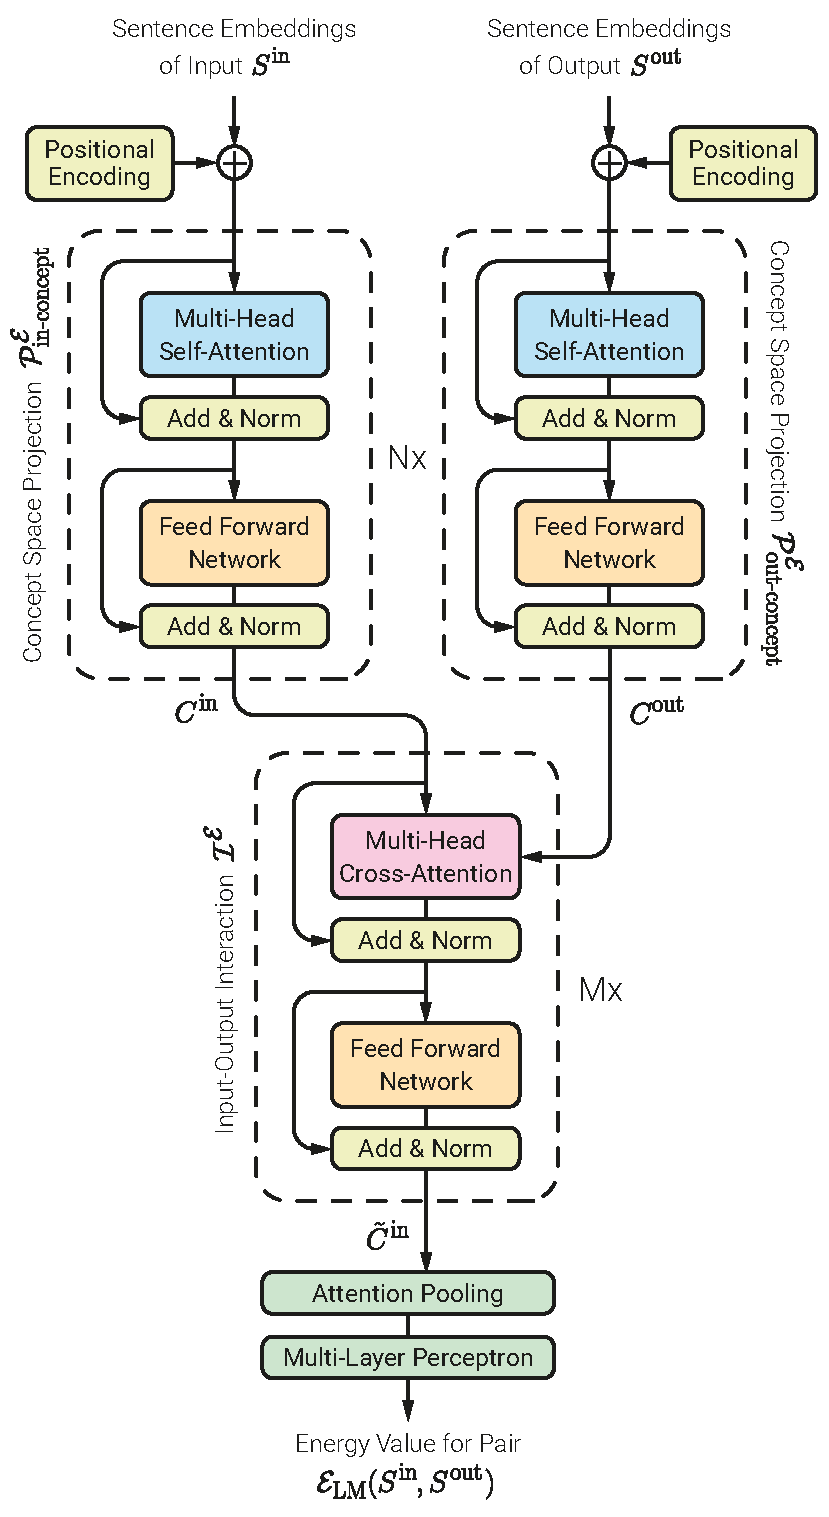
\includegraphics[width=0.45\textwidth]{figures/Fig-EBM-Architecture-V4.pdf}
    \caption{معماری شبکه‌ی جانشین مبتنی بر انرژی ($\mathcal{E}_{\text{\lr{LM}}}$)}\label{fig:chap4_architecture_energy}
\end{figure}

پیش از ورود به ماژول‌های اصلی، از آنجا که مدل‌سازی ما در سطح جملات انجام می‌شود و ترتیب گزاره‌ها در درک بافتار متن نقشی اساسی ایفا می‌کند، ابتدا مانند ترنسفورمر استاندارد طبق بخش~\ref{sec:2-2} یک لایه‌ی رمزگذاری موقعیتی به ماتریس‌های خام افزوده می‌گردد تا اطلاعات ترتیبی حفظ شود:
\begin{align}
    \tilde{S}^{\text{\lr{in}}} &= S^{\text{\lr{in}}} + E_{\text{\lr{pos}}}^{\text{\lr{in}}} \label{eq:chap4_pos_enc_in} \\
    \tilde{S}^{\text{\lr{out}}} &= S^{\text{\lr{out}}} + E_{\text{\lr{pos}}}^{\text{\lr{out}}} \label{eq:chap4_pos_enc_out}
\end{align}
پس از این گام آماده‌سازی، جریان محاسبات در سه مرحله‌ی تصویرسازی فضای مفهومی، تعامل ورودی-خروجی و محاسبه‌ی انرژی انجام می‌شود.

\paragraph{۱. تصویرسازی فضای مفهومی.}
در گام نخست، تانسورهای ورودی ($\tilde{S}^{\text{\lr{in}}}$ و $\tilde{S}^{\text{\lr{out}}}$) به‌عنوان ورودی به دو ماژول خودتوجهی مجزا، یعنی $\mathcal{P}_{\text{\lr{in-concept}}}^{\mathcal{E}}$ و $\mathcal{P}_{\text{\lr{out-concept}}}^{\mathcal{E}}$ تغذیه می‌شوند. دلیل تعبیه‌ی این مرحله‌ی میانی، محدودیت‌های بازنمایی ایستا در غیاب بافتار است.

پژوهش‌های انجام‌شده در مدل‌های مفهومی بزرگ~\cite{lcmteam2024lcm} نشان داده‌اند که مدل‌سازی روابط معنایی می‌تواند با دقت مناسب در فضای پیوسته‌ی تعبیه‌های جمله‌ای انجام پذیرد و نیازی به درگیری با فرم خرد توکن‌ها نیست. همان‌طور که در پژوهش خطیر و همکاران (۲۰۲۵)~\cite{khatir2025aligned} تبیین شد، تعبیه‌های ایستا (مانند خروجی شبکه‌ای نظیر \lr{Sentence-BERT}) از همان ابتدا دارای یک ساختار گروه‌بندی غنی هستند و هم‌تراز در مبدأ محسوب می‌شوند. این ویژگی به ما اجازه می‌دهد تا از این بردارها به‌عنوان یک نقطه‌ی شروع قابل‌اتکا استفاده کنیم. با این وجود، تعبیه‌های ایستا مفاهیم را صرفاً در انزوا مدل می‌کنند. همان‌گونه که پارک و همکاران (۲۰۲۴)~\cite{park2024emergence} در تحلیل دینامیک مفاهیم نشان دادند، مفاهیم در بستر یک بافتار مشخص به‌صورت پویا با یکدیگر تعامل دارند و این فضای مفهومی، دارای وابستگی‌هایی است که فراتر از شباهت معنایی خام هستند.

ماژول‌های تصویرساز فضای مفهومی با در نظر گرفتن این ظرایف طراحی شده‌اند. هر یک از این دو ماژول، شامل $N$ لایه از بلوک‌های استاندارد رمزگذار ترنسفورمر (شامل مکانیزم توجه چندسره و شبکه‌های پیش‌خور همراه با اتصالات باقیمانده و نرمال‌سازی لایه‌ای) هستند. این ماژول‌ها مفاهیم ایستای اولیه را دریافت کرده و با استفاده از مکانیزم خودتوجهی، به جملات اجازه می‌دهند تا برای درک دقیق‌تر معنای خود، به سایر جملات موجود در همان پرامپت (یا پاسخ) توجه کنند. این فرایند زمینه‌سازی بافتاری، بازنمایی هر گزاره را پیش از ارزیابی تعامل متقاطع غنی‌سازی می‌کند و در نتیجه، تعبیه‌های اولیه را به یک فضای مفهومی پویا نگاشت می‌نماید:
\begin{align}
    C^{\text{\lr{in}}} &= \mathcal{P}_{\text{\lr{in-concept}}}^{\mathcal{E}}(\tilde{S}^{\text{\lr{in}}}) \label{eq:chap4_concept_in} \\
    C^{\text{\lr{out}}} &= \mathcal{P}_{\text{\lr{out-concept}}}^{\mathcal{E}}(\tilde{S}^{\text{\lr{out}}}) \label{eq:chap4_concept_out}
\end{align}

\paragraph{۲. تعامل ورودی-خروجی.}
پس از آنکه مفاهیم ورودی و خروجی در بافتار مستقل خود زمینه‌سازی شدند، ضرورت دارد تا میزان انطباق‌پذیری ساختاری و معنایی میان پرامپت و پاسخ ارزیابی شود. در این مرحله، از یک ماژول تعاملی ($\mathcal{I}^{\mathcal{E}}$) مبتنی بر توجه متقاطع استفاده می‌گردد. طراحی این بلوک بر پایه‌ی یافته‌های باتاچاریا و همکاران (۲۰۲۱)~\cite{bhattacharyya2021reranking} استوار است؛ آن‌ها در ارزیابی مدل‌های رتبه‌بندی انرژی نشان دادند که مدل‌هایی که انرژی را صرفاً بر اساس بررسی جمله‌ی خروجی در انزوا محاسبه می‌کنند (مدل‌های انرژی حاشیه‌ای)، در ارزیابی وابستگی‌ها با افت عملکرد مواجه می‌شوند؛ در حالی که مدل‌های انرژی مشترک\enfootnote{joint energy models} که ترکیب ورودی و خروجی را به‌طور هم‌زمان داوری می‌کنند، دقت بسیار بالاتری دارند.

ماژول تعامل ورودی-خروجی ما، که از $M$ لایه از بلوک‌های توجه متقاطع تشکیل شده است، پیاده‌سازی همین ارزیابی مشترک است. هر یک از این لایه‌ها علاوه بر مکانیزم توجه، مجهز به شبکه‌های پیش‌خور، اتصالات باقیمانده و لایه‌های نرمال‌سازی هستند. مطابق با جریان اطلاعات در شکل~\ref{fig:chap4_architecture_energy}، در این ماژول، مفاهیم پویای پرامپت ($C^{\text{\lr{in}}}$) در نقش بردارهای پرسمان ($Q$)، و مفاهیم پویای پاسخ ($C^{\text{\lr{out}}}$) در نقش بردارهای کلید ($K$) و ارزش ($V$) عمل می‌کنند. این مکانیزم به مفاهیم ورودی اجازه می‌دهد تا با مفاهیم خروجی تعامل کرده و بررسی کنند که گزاره‌های پرامپت تا چه میزان با پاسخ تولیدشده انطباق دارند. خروجی این بلوک، نسخه‌ی به‌روزرسانی‌شده‌ای از بازنمایی پرامپت است که آگاهی کاملی از تعاملات خود با پاسخ مدل دارد:
\begin{equation}\label{eq:chap4_cross_attention_interaction}
    \tilde{C}^{\text{\lr{in}}} = \mathcal{I}^{\mathcal{E}}\big(Q=C^{\text{\lr{in}}}, K=C^{\text{\lr{out}}}, V=C^{\text{\lr{out}}}\big)
\end{equation}

\paragraph{۳. محاسبه‌ی انرژی.}
در گام نهایی، اطلاعات تعاملی توزیع‌شده در ماتریس $\tilde{C}^{\text{\lr{in}}}$ باید در قالب یک امتیاز اسکالر یکپارچه شود. معماری این بخش از متمایزگر ترنسفورمری در چارچوب \lr{EBM} بختیین و همکاران (۲۰۱۹)~\cite{bakhtin2019realfake} الهام گرفته شده است، با این تفاوت که با خروجی‌های ساختاریافته‌ی بلوک‌های پیشین تغذیه می‌شود.

از آنجا که هدف ما استخراج یک عدد منفرد (اسکالر انرژی) است، نیازمند عبور داده‌ها از یک شبکه‌ی عصبی پیش‌خور (\lr{MLP}) هستیم. با این وجود، خروجی بلوک تعاملی یک ماتریس دوبعدی از تعبیه‌های متنی با ابعاد $N_{\text{\lr{max}}} \times d$ است. برای فشرده‌سازی اصولی اطلاعات در طول بُعد دنباله بدون از دست دادن وزن متغیر جملات، از یک لایه‌ی تجمیع مبتنی بر توجه\enfootnote{attention pooling} استفاده می‌شود. این عملگر به مدل اجازه می‌دهد تا برخلاف تجمیع میانگین ساده، وزن بیشتری به جملاتی اختصاص دهد که حامل وابستگی تعاملی و معنایی قوی‌تری در بازنمایی نهایی هستند و در نهایت، ماتریس جملات را به یک بردار متراکم واحد ($\mathbf{h}_{\text{\lr{pool}}} \in \mathbb{R}^d$) تقلیل دهد:
\begin{equation}\label{eq:chap4_attention_pooling}
    \mathbf{h}_{\text{\lr{pool}}} = \text{\lr{AttentionPooling}}(\tilde{C}^{\text{\lr{in}}})
\end{equation}
سپس، این بردار فشرده به یک شبکه‌ی عصبی پیش‌خور تمام‌متصل (\lr{MLP}) تغذیه می‌شود تا ویژگی‌ها به یک عدد منفرد تصویر شوند. این عدد اسکالر نهایی، همان انرژی محاسبه‌شده ($\mathcal{E}_{\text{\lr{LM}}}$) است که نشان می‌دهد با توجه به چشم‌انداز انرژی تقریب‌زده‌شده از مدل جعبه‌سیاه، جفت پرامپت و پاسخ تا چه میزان با یکدیگر انطباق دارند:
\begin{equation}\label{eq:chap4_energy_calc}
    \mathcal{E}_{\text{\lr{LM}}}(\mathbf{x}, \mathbf{y}; \theta) = \text{\lr{MLP}}(\mathbf{h}_{\text{\lr{pool}}})
\end{equation}
با فرمول‌بندی این معماری پیش‌رو، در بخش بعدی به چگونگی آموزش این شبکه و تنظیم وزن‌های $\theta$ از طریق توابع زیان تقابلی خواهیم پرداخت.


\subsection{استراتژی پیش‌آموزش و تابع زیان دوگانه}\label{sec:4-3-2}

پس از طراحی معماری شبکه‌ی انرژی، مهم‌ترین چالش در استقرار این مدل جانشین، بهینه‌سازی و آموزش آن است. همان‌گونه که در بخش~\ref{sec:2-4-2} تبیین شد، آموزش مستقیم مدل‌های مبتنی بر انرژی بر روی فضای گسسته‌ی متنی از طریق کمینه‌سازی زیان درست‌نمایی، به دلیل محاسبه‌ناپذیری تابع افراز در فضاهای نامتناهی با بن‌بست ریاضی مواجه است؛ لذا طراحی تابع زیان و استراتژی نمونه‌برداری مناسب برای شبکه‌های انرژی از اساسی‌ترین بخش‌های استقرار مؤثر آن‌هاست. برای عبور از این محدودیت ساختاری و در هماهنگی با رویکردهای یادگیری انرژی پیرو بخش~\ref{sec:2-4-4}، چارچوب \lr{ESCI} از یادگیری تقابلی بهره می‌برد تا بدون نیاز به مدل‌سازی صریح تمامی خروجی‌های ممکن، چشم‌انداز انرژی را شکل دهد.

در انتخاب نوع تابع زیان تقابلی، ما به یافته‌های دنگ و همکاران (۲۰۲۰)~\cite{deng2020residual} و بختیین و همکاران (۲۰۲۱)~\cite{bakhtin2021residual} استناد کرده‌ایم که نشان دادند استفاده از توابع حاشیه‌ای کلاسیک در فضاهای زبانی غالباً با ناپایداری در آموزش مدل‌های انرژی همراه است. بر این اساس، استفاده از استراتژی‌های مبتنی بر تخمین تقابلی نویز (\lr{NCE})~\cite{gutmann2010noise} راهکاری پایدار برای اجتناب از محاسبه‌ی صریح تابع افراز در پردازش زبان به‌شمار می‌رود.

با این وجود، متدولوژی ما در پیاده‌سازی این رویکرد متمایز از ساختارهای پسماند مرسوم است. در پژوهش‌های دنگ و بختیین، مدل انرژی در قالب یک معماری پسماند و با استفاده از \lr{NCE} دودویی آموزش می‌بیند که در آن توزیع نویز مستقیماً توسط توزیع احتمالات یک مدل زبانی خودهمبسته تأمین می‌گردد. اما در رژیم دسترسی جعبه‌سیاه در چارچوب \lr{ESCI}، ما فاقد دسترسی به توزیع احتمالات و لوجیت‌های مدل هدف هستیم. از این رو، ما از تعمیم چندکلاسه‌ی این رویکرد یعنی \lr{InfoNCE}~\cite{oord2018representation} (که در بخش~\ref{sec:2-4-5} تشریح شد) بهره برده‌ایم. استفاده از \lr{InfoNCE} به ما اجازه می‌دهد تا یک نمونه‌ی مثبت را به‌صورت هم‌زمان در برابر $K$ نمونه‌ی منفی ساختاریافته قرار دهیم و پایداری محاسباتی آموزش را بدون وابستگی به توزیع‌های احتمالی درونی تأمین نماییم.

\begin{figure}[ht]
    \centering
    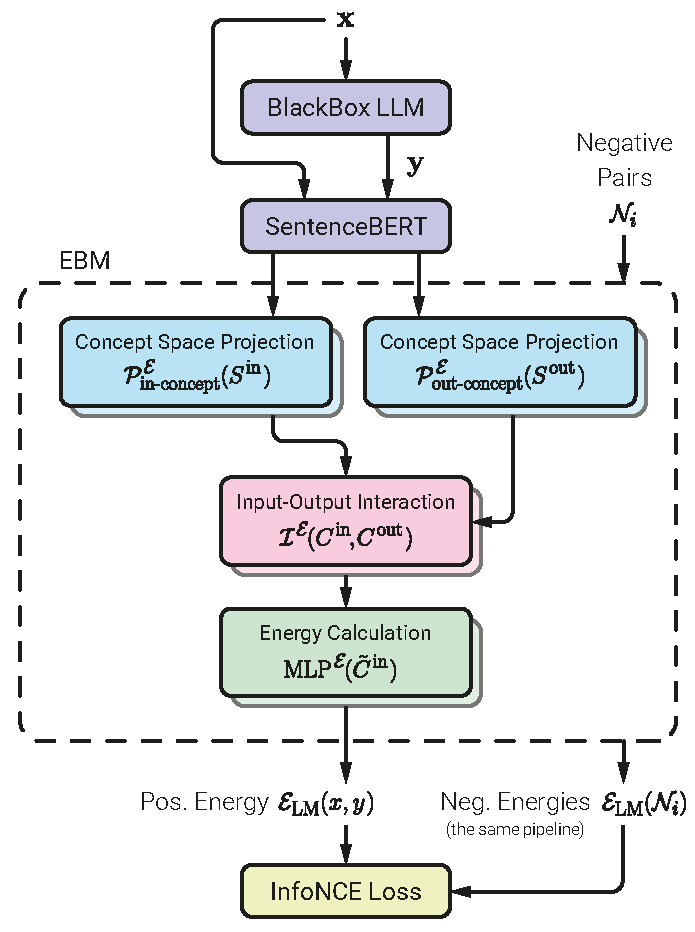
\includegraphics[width=0.5\textwidth]{figures/Fig-EBM-Pretraining-Pipeline-V4.pdf}
    \caption{خط‌لوله‌ی پیش‌آموزش شبکه‌ی جانشین مبتنی بر انرژی ($\mathcal{E}_{\text{\lr{LM}}}$)}\label{fig:chap4_pipeline_energy_pretraining}
\end{figure}

با فرض اینکه جفت منطبق و مثبت ما برای نمونه‌ی $i$ام به‌صورت $(\mathbf{x}_i, \mathbf{y}_i)$ تعریف شود، مجموعه‌ای متشکل از $K$ نمونه‌ی منفی متناظر با همین جفت را به‌صورت $\mathcal{N}_i = \{(\mathbf{x}'_1, \mathbf{y}'_1), \dots, (\mathbf{x}'_K, \mathbf{y}'_K)\}$ در نظر می‌گیریم. برای انسجام، یک تابع امتیازدهی مبتنی بر انرژی به فرم $h(\mathbf{x}, \mathbf{y}) = \exp(-\mathcal{E}_{\text{\lr{LM}}}(\mathbf{x}, \mathbf{y};\theta) / \tau)$ تعریف می‌گردد که در آن $\mathcal{E}_{\text{\lr{LM}}}$ خروجی اسکالر شبکه‌ی انرژی و $\tau > 0$ پارامتر دما است. پارامتر دما به‌عنوان مقیاس‌دهنده‌ی هندسی عمل کرده و حساسیت شبکه به اختلاف میان سطوح انرژی را تنظیم می‌نماید. بر این اساس، تابع زیان تقابلی برای نمونه‌ی $i$ام به‌صورت زیر فرمول‌بندی می‌شود:
\begin{equation}\label{eq:chap4_infonce_base}
    \mathcal{L}_i = -\log \left( \frac{h(\mathbf{x}_i, \mathbf{y}_i)}{h(\mathbf{x}_i, \mathbf{y}_i) + \sum_{(\mathbf{x}', \mathbf{y}') \in \mathcal{N}_i} h(\mathbf{x}', \mathbf{y}')} \right)
\end{equation}
این معادله نشان می‌دهد که مدل با کمینه‌سازی $\mathcal{L}_i$، در تلاش است تا نسبت امتیاز نمونه‌ی مثبت را در برابر مجموع امتیازات تمامی گزینه‌ها بیشینه سازد. برای تعمیم این روند به کل مجموعه‌داده، زیان نهایی برای دسته‌ای به اندازه‌ی $B$ برابر با میانگین زیان‌های انفرادی است:
\begin{equation}\label{eq:chap4_infonce_batch}
    \mathcal{L}_{\text{\lr{batch}}} = \frac{1}{B} \sum_{i=1}^{B} \mathcal{L}_i
\end{equation}

ساختار اجرایی این فرایند بهینه‌سازی در شکل~\ref{fig:chap4_pipeline_energy_pretraining} نشان داده شده است. پرامپت خام ابتدا به مدل زبانی جعبه‌سیاه ارسال شده تا پاسخ واقعی تولید گردد. این جفت، پس از تبدیل به بردار توسط شبکه‌ی تعبیه‌ساز، وارد جریان محاسباتی مدل انرژی شده و در نهایت، انرژی اسکالر دریافت می‌کند. هم‌زمان، مجموعه‌ی نمونه‌های منفی ($\mathcal{N}_i$) نیز از همین خط‌لوله عبور کرده و مقادیر انرژی متناظر را تولید می‌نمایند. در گام نهایی، این مقادیر وارد تابع زیان \lr{InfoNCE} می‌شوند تا انرژی جفت‌های واقعی کاهش و انرژی جفت‌های نامنطبق افزایش یابد.

کیفیت چشم‌انداز انرژی حاصل از این خط‌لوله، وابسته به طراحی مجموعه‌ی منفی ($\mathcal{N}_i$) است. ما برای اینکه شبکه‌ی انرژی بتواند هم‌زمان ویژگی‌های آماری کلان و وابستگی‌های ساختاری گزاره‌ای را بیاموزد، تابع زیان نهایی را به‌صورت یک ساختار دوگانه متشکل از دو هدف مکمل طراحی کرده‌ایم:

\paragraph{۱. زیان وفاداری سراسری ($\mathcal{L}_{\text{\lr{fidelity}}}$).}
هدف از این تابع زیان، وادار کردن شبکه به یادگیری الگوهای سبکی و توزیعی خروجی‌های مدل هدف است؛ به‌گونه‌ای که مدل جانشین بیاموزد خروجی‌های واقعی جعبه‌سیاه را از متون تولیدشده در سایر توزیع‌ها متمایز کند. این بخش از تابع زیان، از معماری \lr{EBM} متمایزگر بختیین و همکاران (۲۰۱۹)~\cite{bakhtin2019realfake} الهام گرفته شده است که نشان دادند یک ترنسفورمر دوسویه می‌تواند با تکیه بر نمونه‌های منفی سراسری (نظیر متون انسانی یا متون حاصل از سایر مدل‌ها)، به ارزیابی توانمند برای سنجش انطباق توزیعی تبدیل شود. 

در این راستا، برای هر نمونه‌ی $i$، دو مجموعه‌ی منفی متمایز در نظر گرفته می‌شود: نخست، پاسخ‌های انسانی از مجموعه‌داده‌ی مرجع ($\mathcal{N}^{\text{\lr{hum}}}_i$)؛ و دوم، پاسخ‌های تولیدشده توسط یک مدل زبانی متفاوت ($\mathcal{N}^{\text{\lr{other}}}_i$). با فرض ثابت بودن پرامپت $\mathbf{x}_i$، مجموعه‌ی کل نمونه‌های منفی وفاداری برابر با $\mathcal{N}^{\text{\lr{fid}}}_i = \mathcal{N}^{\text{\lr{hum}}}_i \cup \mathcal{N}^{\text{\lr{other}}}_i$ است. در نتیجه، تابع زیان وفاداری برای نمونه‌ی $i$ام به‌صورت زیر می‌باشد:
\begin{equation}\label{eq:chap4_loss_fidelity}
    \mathcal{L}_{\text{\lr{fidelity}}}^{(i)} = -\log \left( \frac{h(\mathbf{x}_i, \mathbf{y}_i)}{h(\mathbf{x}_i, \mathbf{y}_i) + \sum_{(\mathbf{x},\mathbf{y}') \in \mathcal{N}^{\text{\lr{fid}}}_i} h(\mathbf{x}, \mathbf{y}')} \right)
\end{equation}
این زیان تضمین می‌کند که چشم‌انداز انرژی در مقیاس کلان، به الگوهای متنی مدل جعبه‌سیاه وفادار بماند و از افت عملکرد در درک فضای سراسری جلوگیری نماید.

\paragraph{۲. زیان وابستگی محلی ($\mathcal{L}_{\text{\lr{dep}}}$).}
اگر شبکه‌ی انرژی صرفاً با زیان وفاداری آموزش ببیند، ممکن است به‌جای کشف ارتباطات محتوایی، به همبستگی‌های سطحی بسنده نماید. برای رفع این نقیصه و وادار کردن مدل به سنجش وابستگی‌های ساختاری میان جملات، زیان وابستگی محلی با استفاده از استراتژی نمونه‌برداری پادواقعی\enfootnote{counterfactual sampling} طراحی شده است.

ایده‌ی کلیدی در این بخش، استفاده از ماسک‌گذاری تصادفی برای ارزیابی جزء‌به‌جزء است. برای سنجش اینکه یک بخش از پاسخ تا چه اندازه به بخش خاصی از پرامپت وابسته است، شبکه‌ی انرژی باید این گزاره‌ها را در شرایطی ارزیابی کند که بخش‌هایی از بافتار متنی حذف شده باشند. به همین منظور، در هر گام پردازش، تعدادی از جملات در پرامپت و پاسخ به‌صورت تصادفی ماسک می‌شوند تا یک پرامپت جزئی ($\mathbf{x}_{\text{\lr{part}}}$) و یک پاسخ جزئی ($\mathbf{y}_{\text{\lr{part}}}$) شکل گیرد.

در دسته‌ای به اندازه‌ی $B$، این هدف آموزشی از دو مکانیزم نمونه‌برداری مستقل بهره می‌برد که هر یک با ساخت مجموعه‌ای از نمونه‌های منفی به اندازه‌ی $K = B-1$ برای نمونه‌ی $i$ام عمل می‌کنند:

نخست، نمونه‌بردار پاسخ جزئی که در آن پرامپت جزئی یک نمونه ($\mathbf{x}_{\text{\lr{part}}, i}$) ثابت نگه‌داشته شده و پاسخ جزئی متناظر با آن ($\mathbf{y}_{\text{\lr{part}}, i}$)، در تقابل با پاسخ‌های جزئی سایر نمونه‌های دسته ($\mathbf{y}'_{\text{\lr{part}}, j}$) قرار می‌گیرد. به‌بیان ریاضی، مجموعه‌ی منفی برای این حالت برابر با $\mathcal{N}^{\text{\lr{resp}}}_i = {\{(\mathbf{x}_{\text{\lr{part}}, i}, \mathbf{y}'_{\text{\lr{part}}, j})\}}_{j=1, j \neq i}^B$ است. این ساختار، مدل را ملزم می‌کند بررسی نماید که آیا خروجی ارائه‌شده با ورودی جزئی همخوانی ساختاری دارد یا خیر. بر اساس فرمول مبنای~\ref{eq:chap4_infonce_base}، تابع زیان برای این نمونه‌بردار به‌صورت زیر محاسبه می‌شود:
\begin{equation}\label{eq:chap4_loss_resp_dep}
    \mathcal{L}_{\text{\lr{resp-dep}}}^{(i)} = -\log \left( \frac{h(\mathbf{x}_{\text{\lr{part}}, i}, \mathbf{y}_{\text{\lr{part}}, i})}{h(\mathbf{x}_{\text{\lr{part}}, i}, \mathbf{y}_{\text{\lr{part}}, i}) + \sum_{(\mathbf{x}', \mathbf{y}') \in \mathcal{N}^{\text{\lr{resp}}}_i} h(\mathbf{x}', \mathbf{y}')} \right)
\end{equation}

دوم، مکانیزم متناظری توسط نمونه‌بردار پرامپت جزئی اجرا می‌شود. در این مکانیزم، پاسخ جزئی نمونه‌ی $i$ام ($\mathbf{y}_{\text{\lr{part}}, i}$) ثابت می‌ماند و در برابر پرامپت‌های جزئی سایر نمونه‌ها ($\mathbf{x}'_{\text{\lr{part}}, j}$) قرار می‌گیرد، به‌گونه‌ای که مجموعه‌ی منفی به فرم $\mathcal{N}^{\text{\lr{pmt}}}_i = {\{(\mathbf{x}'_{\text{\lr{part}}, j}, \mathbf{y}_{\text{\lr{part}}, i})\}}_{j=1, j \neq i}^B$ تشکیل می‌گردد. این تقابل تضمین می‌کند که شبکه می‌تواند خروجی را مستقیماً به پیش‌آیندهای متناظر در ورودی متصل سازد:
\begin{equation}\label{eq:chap4_loss_pmt_dep}
    \mathcal{L}_{\text{\lr{pmt-dep}}}^{(i)} = -\log \left( \frac{h(\mathbf{x}_{\text{\lr{part}}, i}, \mathbf{y}_{\text{\lr{part}}, i})}{h(\mathbf{x}_{\text{\lr{part}}, i}, \mathbf{y}_{\text{\lr{part}}, i}) + \sum_{(\mathbf{x}', \mathbf{y}') \in \mathcal{N}^{\text{\lr{pmt}}}_i} h(\mathbf{x}', \mathbf{y}')} \right)
\end{equation}

از آنجا که هر یک از این دو نمونه‌بردار محور متفاوتی از داده‌ها را تغییر می‌دهند (یکی پرامپت و دیگری پاسخ را در برابر نویز قرار می‌دهد)، زیان کلی وابستگی محلی برای نمونه‌ی $i$ام از حاصل‌جمع این دو زیان به‌دست می‌آید:
\begin{equation}\label{eq:chap4_loss_dep_total}
    \mathcal{L}_{\text{\lr{dep}}}^{(i)} = \mathcal{L}_{\text{\lr{resp-dep}}}^{(i)} + \mathcal{L}_{\text{\lr{pmt-dep}}}^{(i)}
\end{equation}

طراحی این بخش، بر دو مبنای نظری استوار است. نخست، همان‌طور که در پژوهش پارک و همکاران (۲۰۲۳)~\cite{park2023thelinear} پیرامون فرضیه‌ی بازنمایی خطی مطرح شد، مفاهیم در فضاهای با ابعاد بالا درهم‌تنیده‌اند و بهره‌گیری از تقابل‌های ساختاریافته روشی مؤثر برای خنثی‌سازی نویز پس‌زمینه و مجزاسازی مؤلفه‌های هدف در فضای بازنمایی است. تضاد تقابلی در فاز آموزش ما، \lr{EBM} را وادار می‌کند تا با قرار دادن یک بافتار ثابت در برابر ادامه‌های نامرتبط، همبستگی‌های سطحی را نادیده گرفته و چشم‌انداز انرژی را بر وابستگی‌های ساختاری متمرکز کند. دوم، پیرو مباحث بخش~\ref{sec:3-1-3-3}، فریدمن و همکاران (۲۰۲۴)~\cite{friedman2024interpretability} نشان دادند که آموزش انحصاری بر روی داده‌های درون‌توزیع می‌تواند به توهم تفسیرپذیری در مواجهه با شرایط جدید بینجامد. نمونه‌بردارهای وابستگی محلی با تکیه بر ماسک‌گذاری و جفت‌سازی‌های متنوع، شبکه‌ی جانشین را با سناریوهای مخدوش و تقلیل‌یافته مواجه می‌سازند تا با یادگیری تفاوت انرژی میان ساختارهای منسجم و ناقص، مدل در برابر خطای تعمیم‌پذیری پایدار بماند.

\paragraph{فرمول‌بندی نهایی تابع زیان.}
همان‌گونه که توسط تو و همکاران (۲۰۲۰)~\cite{tu2020improving} اشاره شد، آموزش مدل‌های مبتنی بر انرژی نیازمند کنترل شکل‌گیری کمینه‌های کاذب انرژی است و رویکردی مؤثر برای مهار آن، استفاده از آموزش دوگانه با اعمال نمونه‌های منفی سخت است. بر همین اساس، تابع زیان کل در چارچوب ما ترکیبی متوازن از دو هدف وفاداری سراسری و وابستگی محلی است. با در نظر گرفتن پارامتر وزنی $\lambda \in [0, 1]$ برای تنظیم توازن میان این دو مؤلفه، تابع بهینه‌سازی نهایی شبکه‌ی انرژی برای یک دسته‌ی کامل به‌صورت زیر تعریف می‌شود:
\begin{equation}\label{eq:chap4_ebm_total_loss}
    \mathcal{L}_{\text{\lr{batch-total}}} = \frac{1}{B} \sum_{i=1}^{B} \left[ (1-\lambda) \mathcal{L}_{\text{\lr{fidelity}}}^{(i)} + \lambda \mathcal{L}_{\text{\lr{dep}}}^{(i)} \right]
\end{equation}

این طراحی دوگانه، پاسخی ساختاریافته به چالش فقدان داده‌های برچسب‌دار برای وابستگی‌های گزاره‌ای است. از نظر تئوریک، روشناس و همکاران (۲۰۱۹)~\cite{rooshenas2019searchguided} نشان دادند که توابع انرژی ساختاریافته می‌توانند بدون نیاز به حقیقت پایه‌ی صریح و با تکیه بر ارزیابی‌های اسکالر هدایت‌گر آموزش ببینند. در شبکه‌ی جانشین ما، متون واقعی مدل هدف نقش لنگرگاه را ایفا کرده و اعمال سیستماتیک اختلالات ساختاریافته، سیگنال آموزشی لازم را فراهم می‌آورد. جزئیات نمونه‌بردارهای منتخب در پیوست~\ref{app:appendix_negative_samplers} ارائه شده است و بررسی تفصیلی رفتار تجربی این مؤلفه‌ها در فصل~\ref{chap:chapter5_experiments} انجام خواهد گرفت.

بدین‌ترتیب، پس از اتمام این فاز از آموزش، یک مدل جانشین ارزیاب در اختیار داریم که الگوهای انطباق‌پذیری متنی و وابستگی‌های گزاره‌ای مدل هدف را به‌صورت کل‌نگر یاد گرفته است و می‌تواند به‌عنوان یک ناظر، سیگنال‌های لازم را برای آموزش شبکه‌ی مفسر در فاز دوم چارچوب فراهم آورد.



\section{فاز دوم: شبکه‌ی مفسر}\label{sec:4-4}

همان‌طور که در فصل پیشین واکاوی شد، چالش بنیادین در روش‌های مبتنی بر اختلال (همانند \lr{LIME} یا \lr{SHAP})، بار محاسباتی سنگین آن‌ها در زمان استنتاج است. جستجو برای یافتن زیرمجموعه‌ی بهینه‌ای از کلمات در میان فضای نمایی پرامپت‌های طولانی، مستلزم استعلام‌های مکرر از مدل جعبه‌سیاه است. در فاز نخست این چارچوب، مدل جانشین مبتنی بر انرژی (\lr{EBM}) با ارائه‌ی یک چشم‌انداز انرژی سراسری، الگوهای انطباق‌پذیری متنی و وابستگی‌های گزاره‌ای میان ورودی و خروجی را تقریب زده است. با این حال، هدف نهایی مسئله‌ی انتساب بر پایه‌ی مسئله‌ی~\ref{prob:chap1_causal_attribution}، یافتن زیرمجموعه‌ی بهینه‌ی جملات پرامپت (در قالب بردار ماسک اهمیت $\mathbf{m}$) است که به‌عنوان پیش‌آیند، بیشترین تأثیر را بر تولید بخش هدف خروجی ($\mathbf{y}_T$) داشته‌اند.

اگر بخواهیم برای یافتن این زیرمجموعه مستقیماً از مدل انرژی استفاده کنیم، باید در زمان استنتاج، تابع انرژی را بر روی تمامی ترکیبات ممکن پرامپت ارزیابی کرده و زیرمجموعه‌ای را بیابیم که انرژی جفت باقیمانده را کمینه می‌سازد:
\begin{equation}\label{eq:chap4_combinatorial_search}
    \mathbf{m}^* = \arg\min_{\mathbf{m} \in {\{0, 1\}}^N} \mathcal{E}_{\text{\lr{LM}}}(\mathbf{x} \odot \mathbf{m}, \mathbf{y}_T; \theta)
\end{equation}
این رویکرد، به دلیل ماهیت گسسته‌ی ماسک دودویی، نیازمند یک جستجوی ترکیبیاتی نمایی ($\mathcal{O}(2^N)$) است و در صورت استفاده از آزادسازی پیوسته نیز، محتاج بهینه‌سازی گرادیانی تکرارشونده برای هر نمونه‌ی جدید خواهد بود؛ امری که کاربردپذیری عملیاتی چنین سیستمی را با محدودیت روبه‌رو می‌سازد.

برای غلبه بر این مانع محاسباتی، فاز دوم چارچوب \lr{ESCI} بر پایه‌ی پارادایم استنتاج مستهلک‌شده~\cite{tu2018learning} طراحی شده است. بر اساس این الگو، به‌جای اجرای جستجوهای پرهزینه در زمان ارزیابی، بار محاسباتی استخراج پیش‌آیندها مستهلک شده و به فاز آموزش منتقل می‌گردد. بدین‌منظور، ما یک شبکه‌ی عصبی مستقل و پیش‌خور به نام مفسر ($\mathcal{IN}$) با پارامترهای قابل‌یادگیری $\alpha$ طراحی می‌کنیم که وظیفه دارد این جستجوی پیچیده را تقریب بزند:
\begin{equation}
    \mathbf{m} = \mathcal{IN}(\mathbf{x}, \mathbf{y}, T; \alpha)
\end{equation}

این شبکه‌ی مفسر آموزش می‌بیند تا دانش توزیع‌شده در چشم‌انداز \lr{EBM} را در پارامترهای خود تقطیر کند. با بهره‌گیری از این سازوکار، شبکه‌ی استنتاج به‌گونه‌ای تنظیم می‌شود که نگاشت مستقیم نمونه به زیرمجموعه‌ی پیش‌آیند بهینه را فرابگیرد. این استقلال ساختاری تضمین می‌کند که در زمان استقرار سیستم، فرایند انتساب ویژگی و شناسایی پیش‌آیندهای اثرگذار، تنها با یک بار عبور پیش‌رو در گراف محاسباتی مفسر و با پیچیدگی زمانی ثابت $\mathcal{O}(1)$ انجام پذیرد.


\subsection{معماری مفسر}\label{sec:4-4-1}

شبکه‌ی مفسر $\mathcal{IN}(\mathbf{x}, \mathbf{y}, T; \alpha)$ به‌عنوان یک مدل استخراج‌گر طراحی شده است که پرامپت کامل ($\mathbf{x} \in \mathcal{S}^N$)، پاسخ کامل تولیدشده ($\mathbf{y} \in \mathcal{S}^M$) و مجموعه‌ی شاخص‌های جملات هدف خروجی ($T \subseteq \{1, \dots, M\}$) را دریافت کرده و با حفظ بافتار کامل خروجی و شرطی‌سازی محاسبات بر روی شاخص‌های هدف $T$، یک بردار ماسک اهمیت دودویی $\mathbf{m} \in {\{0, 1\}}^N$ (و در حین آموزش، ماسک پیوسته $\hat{\mathbf{m}} \in {(0, 1)}^N$) تولید می‌کند. ساختار کلی این شبکه در شکل~\ref{fig:chap4_architecture_interpreter} به تصویر کشیده شده است.

\begin{figure}[ht]
    \centering
    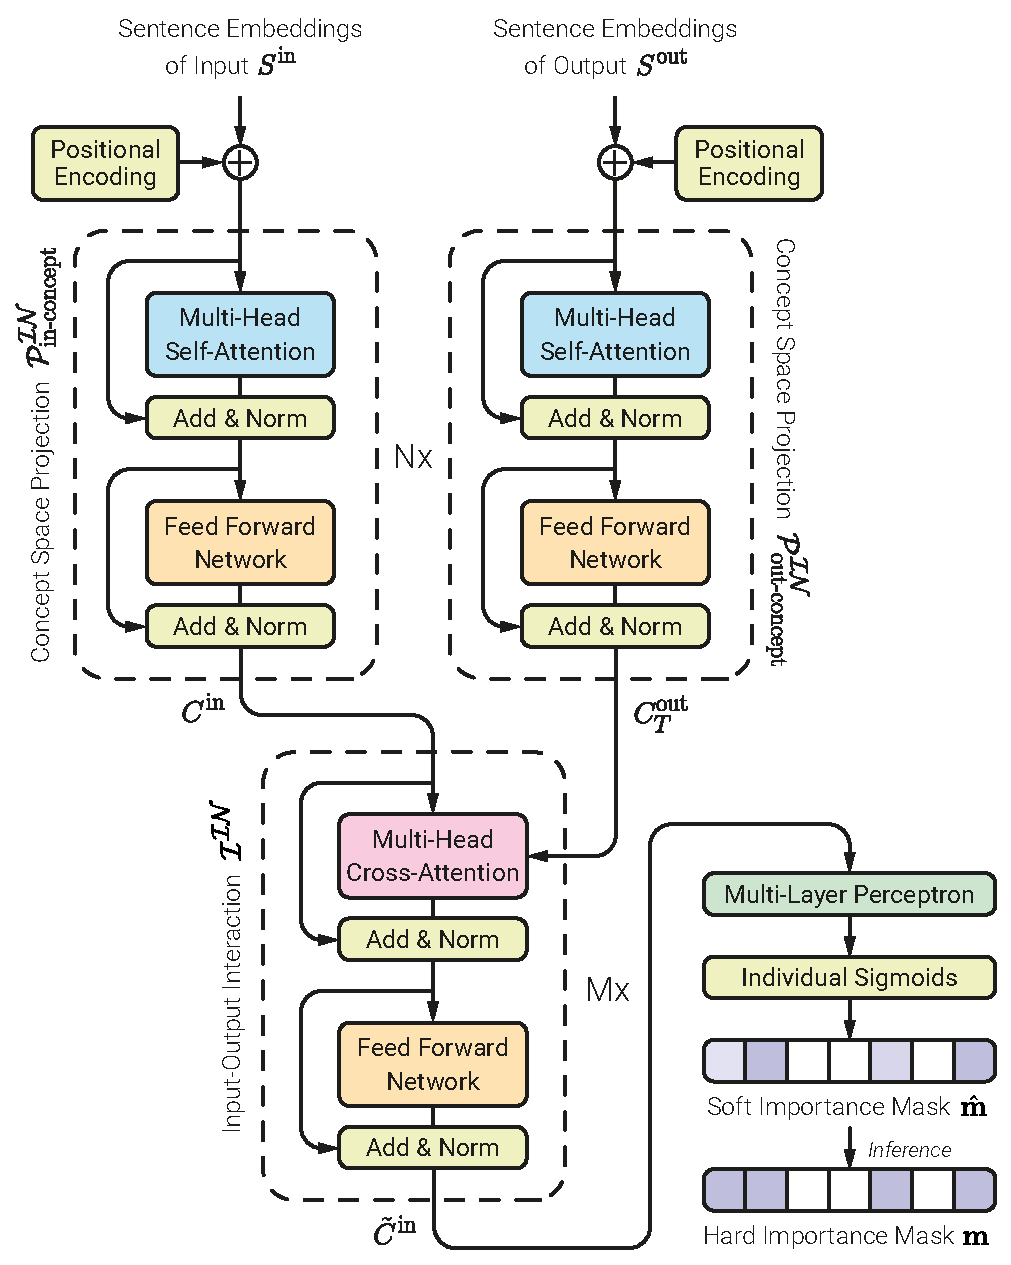
\includegraphics[width=0.6\textwidth]{figures/Fig-Interpreter-Architecture-V4.pdf}
    \caption{معماری شبکه‌ی مفسر ($\mathcal{IN}$)}\label{fig:chap4_architecture_interpreter}
\end{figure}

معماری این مفسر، ساختار سه‌مرحله‌ای مدل \lr{EBM} (بخش~\ref{sec:4-3-1}) را بازتاب می‌دهد و از یک ترنسفورمر دوسویه بهره می‌برد؛ اما تغییرات مشخصی در آن اعمال شده است تا از یک ارزیاب کلان به یک انتخاب‌گر پیش‌آیند با هدایت هدفمند تبدیل شود. جریان محاسبات در این معماری شامل مراحل زیر است:

\paragraph{۱. تصویرسازی فضای مفهومی.}
همانند مدل انرژی، پیش از هر پردازشی، یک لایه‌ی رمزگذاری موقعیتی به ماتریس‌های تعبیه‌ی ورودی و خروجی اضافه می‌شود تا اطلاعات ترتیبی حفظ گردد:
\begin{align}
    \tilde{S}^{\text{\lr{in}}} &= S^{\text{\lr{in}}} + E_{\text{\lr{pos}}}^{\text{\lr{in}}} \label{eq:chap4_interp_pos_enc_in} \\
    \tilde{S}^{\text{\lr{out}}} &= S^{\text{\lr{out}}} + E_{\text{\lr{pos}}}^{\text{\lr{out}}} \label{eq:chap4_interp_pos_enc_out}
\end{align}
سپس، این تعبیه‌ها از طریق ماژول‌های خودتوجهی به یک فضای مفهومی پویا تصویر می‌شوند. این دو ماژول تصویرساز مفسر ($\mathcal{P}_{\text{\lr{in-concept}}}^{\mathcal{IN}}$ و $\mathcal{P}_{\text{\lr{out-concept}}}^{\mathcal{IN}}$) از نظر معماری مشابه همتایان خود در \lr{EBM} طراحی شده‌اند (شامل $N$ لایه‌ی استاندارد ترنسفورمر). با این حال، پارامترهای ماژول‌ها در شبکه‌ی مفسر ($\alpha$) کاملاً از وزن‌های شبکه‌ی \lr{EBM} ($\theta$) مستقل بوده و منحصراً برای وظیفه‌ی استخراج ویژگی آموزش می‌بینند:
\begin{align}
    C^{\text{\lr{in}}} &= \mathcal{P}_{\text{\lr{in-concept}}}^{\mathcal{IN}}(\tilde{S}^{\text{\lr{in}}}) \label{eq:chap4_interp_concept_in} \\
    C^{\text{\lr{out}}} &= \mathcal{P}_{\text{\lr{out-concept}}}^{\mathcal{IN}}(\tilde{S}^{\text{\lr{out}}}) \label{eq:chap4_interp_concept_out}
\end{align}
از منظر طراحی معماری، هم‌سان‌سازی تعداد لایه‌های این ماژول‌ها با تصویرسازهای شبکه‌ی \lr{EBM} و استفاده از وزن‌های تصویرساز مدل انرژی برای مقداردهی اولیه‌ی تصویرساز مفسر، انتقال بازنمایی‌های مفهومی اولیه را تسهیل کرده و روند یادگیری مفسر را در استخراج ویژگی‌ها هموار می‌سازد.

\paragraph{۲. ماسک‌گذاری هدف و تعامل متمرکز.}
نقطه‌ی افتراق کلیدی مفسر با شبکه‌ی \lr{EBM}، در بلوک تعاملی آن‌ها نهفته است. در مدل انرژی، نیازمند ارزیابی انطباق‌پذیری کل پرامپت با کل پاسخ برای سنجش الگوهای کلان بودیم؛ اما در شبکه‌ی مفسر، تحلیل‌گر در پی شناسایی پیش‌آیندهای اثرگذار بر گزاره‌های معینی از خروجی ($T$) است. با این حال، مفسر نیازمند دریافت بافتار کامل پاسخ ($\mathbf{y}$) در بازنمایی‌های مفهومی خود است تا ساختار کلی متن حفظ شود.

بدین‌منظور، پیش از ورود به بلوک توجه متقاطع، شرطی‌سازی بر روی زیرمجموعه‌ی هدف از طریق اعمال بردار شاخص دودویی $\mathbf{m}_T \in {\{0, 1\}}^{N_{\text{\lr{max}}}}$ بر روی تانسور مفاهیم خروجی محقق می‌شود (که در آن به ازای $j \in T$ مقدار ۱ و در غیر این صورت ۰ قرار می‌گیرد):
\begin{equation}
    C^{\text{\lr{out}}}_T = \mathbf{m}_T \odot C^{\text{\lr{out}}} \label{eq:chap4_target_masking}
\end{equation}
سپس، تانسورهای $C^{\text{\lr{in}}}$ و $C^{\text{\lr{out}}}_T$ به ماژول تعاملی مفسر ($\mathcal{I}^{\mathcal{IN}}$) متشکل از $M$ لایه از بلوک‌های توجه متقاطع تغذیه می‌شوند. در این تقاطع، مفاهیم ورودی ($C^{\text{\lr{in}}}$) در نقش بردارهای پرسمان ($Q$)، و مفاهیم شرطی‌شده‌ی هدف ($C^{\text{\lr{out}}}_T$) در نقش بردارهای کلید ($K$) و ارزش ($V$) قرار می‌گیرند:
\begin{equation}\label{eq:chap4_interp_interaction}
    \tilde{C}^{\text{\lr{in}}} = \mathcal{I}^{\mathcal{IN}}\big(Q=C^{\text{\lr{in}}}, K=C^{\text{\lr{out}}}_T, V=C^{\text{\lr{out}}}_T\big)
\end{equation}
این ساختار به مفسر امکان می‌دهد تا ضمن بهره‌مندی از بافتار کامل پاسخ در لایه‌های پیشین، تمرکز توجه متقاطع را منحصراً معطوف به گزاره‌های هدف نموده و بازنمایی‌های پرامپت را بر پایه‌ی وابستگی به شاخص‌های $T$ به‌روزرسانی کند. در نتیجه، خروجی این بلوک ($\tilde{C}^{\text{\lr{in}}}$)، حاوی اطلاعات متمرکز بر تولید گزاره‌های هدف خواهد بود.

\paragraph{۳. استخراج امتیازات محلی.}
در گام بعدی، به‌جای فشرده‌سازی اطلاعات تمامی جملات به یک اسکالر واحد با استفاده از تجمیع مبتنی بر توجه، در مفسر نیازمند تولید یک خروجی مجزا به ازای تک‌تک جملات پرامپت هستیم تا درباره‌ی انتساب هر گزاره تصمیم‌گیری شود.

بدین‌منظور، خروجی بلوک توجه متقاطع ($\tilde{C}^{\text{\lr{in}}}$) مستقیماً به یک شبکه‌ی پرسپترون چندلایه‌ی کوچک (\lr{MLP}) با بعد خروجی ۱ تغذیه می‌شود. این لایه به‌صورت توزیع‌شده بر روی بازنمایی هر موقعیت (هر جمله‌ی ورودی) به‌طور مستقل عمل می‌کند. خروجی این لایه، برداری از امتیازات خام یا لوجیت‌ها است ($\mathbf{z} \in \mathbb{R}^{N_{\text{\lr{max}}}}$) که نشان‌دهنده‌ی اهمیت اولیه‌ی هر جمله‌ی پرامپت در ارتباط با خروجی هدف است:
\begin{equation}\label{eq:chap4_interp_logits}
    \mathbf{z} = \text{\lr{MLP}}(\tilde{C}^{\text{\lr{in}}})
\end{equation}

\paragraph{۴. آزادسازی پیوسته و تقریب توزیع مستقل.}
برای تبدیل این امتیازات به یک انتخاب گسسته (ماسک اهمیت دودویی $\mathbf{m}$)، نیازمند یک عملگر مشتق‌پذیر هستیم تا شبکه‌ی مفسر بتواند در طی فرایند پس‌انتشار آموزش ببیند. در روش‌های پایه‌ی انتخاب ویژگی نظیر \lr{L2X}~\cite{chen2018learning}، از عملگر گامبل-سافت‌مکس استفاده می‌شود. این عملگر با فرض وجود یک بودجه‌ی احتمالی ثابت (مجموع احتمالات برابر ۱)، ویژگی‌ها را مجبور به رقابت در یک توزیع دسته‌بندی می‌کند و زیرمجموعه‌ای با اندازه‌ی ازپیش‌تعیین‌شده را برمی‌گزیند.

با این وجود، تحلیل ساختاری نشان می‌دهد که اعمال سافت‌مکس در این بستر با چالش‌های نظری و هندسی روبه‌رو است. از منظر نظری، عملگر سافت‌مکس برای مدل‌سازی دسته‌های مانعه‌الجمع طراحی شده است؛ در حالی که در پردازش زبان طبیعی، مفاهیم غالباً در چندین گزاره توزیع شده و نیازمند ارزیابی غیررقابتی و چندگانه هستند~\cite{stahlberg2022jam}. علاوه بر این، محدودیت ساختاری تنگنای سافت‌مکس~\cite{yang2018breaking} نشان می‌دهد که این عملگر به دلیل محدودیت‌های رتبه‌ی ماتریس در فضای پنهان، ظرفیت بازنمایی توزیع‌های واژگانی چندوجهی را ندارد~\cite{chang2022softmax}.

فراتر از این محدودیت‌های نظری، در معماری حاضر، ترکیب این قید رقابتی با مکانیزم توجه متقاطع به افت مقیاس بردارها می‌انجامد. هنگامی که سافت‌مکس بودجه‌ی احتمالی را میان چندین جمله‌ی گزینش‌شده تقسیم می‌کند، مقیاس بردار تعبیه‌ی هر جمله تقلیل می‌یابد. این کاهش مقیاس، در ورود به لایه‌ی توجه متقاطع شبکه‌ی انرژی، تمرکز محاسبات را تضعیف کرده و سبب می‌شود \lr{EBM} (که با بردارهای استاندارد آموزش دیده است) مقادیر نامتعارفی تولید کند. در نتیجه، الگوریتم بهینه‌ساز برای اجتناب از این تغییر مقیاس، مفسر را به سوی تخصیص تمام وزن به یک جمله‌ی منفرد سوق می‌دهد. اثبات تحلیلی و جزئیات ریاضی این پدیده در پیوست~\ref{app:appendix_softmax_bottleneck} ارائه شده است.

برای غلبه بر این چالش، در متدولوژی \lr{ESCI} از مدل‌سازی رقابتی عبور کرده و فرایند انتخاب را به‌عنوان مجموعه‌ای از توزیع‌های برنولی\enfootnote{Bernoulli distribution} مستقل مدل‌سازی کرده‌ایم. بدین‌منظور، بردار لوجیت‌ها وارد یک تابع سیگموئید می‌شود تا امتیاز هر جمله به‌صورت مجزا به بازه‌ی $(0, 1)$ نگاشت گردد:
\begin{equation}\label{eq:chap4_interp_sigmoid}
    \hat{\mathbf{m}} = \text{\lr{Sigmoid}}(\mathbf{z})
\end{equation}
این بردار احتمالات پیوسته ($\hat{\mathbf{m}}$)، همان ماسک نرم است که در فاز آموزش، مستقیماً بر روی تعبیه‌های ورودی اعمال می‌شود و امکان جریان هموار گرادیان‌ها را بدون تخریب مقیاس هندسی بردارها فراهم می‌سازد.

در فاز استنتاج، برای تولید ماسک سخت ($\mathbf{m}$)، با در نظر گرفتن یک حد آستانه‌ی کوچک ($\epsilon$)، جملاتی که امتیازشان بالاتر از این آستانه باشد انتخاب شده و درایه‌های معادل آن‌ها برابر با ۱ قرار می‌گیرند:
\begin{equation}\label{eq:chap4_interp_hard_mask}
    \mathbf{m} = \mathbb{I}(\hat{\mathbf{m}} > \epsilon)
\end{equation}

طراحی این شبکه‌ی مفسر مستقل که به‌صورت قطعی و در زمان‌ثابت یک بردار ماسک تولید می‌کند، از نظر ساختاری الهام‌گرفته از چارچوب \lr{L2X}~\cite{chen2018learning} است. با این تفاوت که به دلیل ماهیت زایا و پیچیده‌ی مدل‌های زبانی، محاسبه‌ی مستقیم اطلاعات متقابل غیرعملی است و در چارچوب \lr{ESCI}، شبکه‌ی مفسر به‌جای بیشینه‌سازی اطلاعات متقابل آماری، آموزش می‌بیند تا شکاف انرژی را در چشم‌انداز \lr{EBM} بهینه‌سازی کند؛ فرایندی که توابع زیان آن در بخش بعد فرمول‌بندی می‌شوند.


\subsection{تابع هدف مفسر}\label{sec:4-4-2}

پس از استخراج ماسک نرم $\hat{\mathbf{m}} = \mathcal{IN}(\mathbf{x}, \mathbf{y}, T; \alpha) \in {(0, 1)}^N$ از شبکه‌ی مفسر، پرامپت اصلی کاربر مطابق با تعاریف~\ref{def:chap1_mask_space} و~\ref{prob:chap1_causal_attribution} در فضای بازنمایی‌ها به دو زیرمجموعه تفکیک می‌شود:
نخست، زیرمجموعه‌ی پیش‌آیندهای اثرگذار گزینش‌شده ($\mathbf{x}_S$):
\begin{equation}
    \mathbf{x}_S = \mathbf{x} \odot \hat{\mathbf{m}}
\end{equation}
و دوم، زیرمجموعه‌ی متمم یا دورریز ($\mathbf{x}_{\text{\lr{discard}}}$) که فاقد وابستگی معنادار به گزاره‌های هدف تلقی می‌گردد:
\begin{equation}
    \mathbf{x}_{\text{\lr{discard}}} = \mathbf{x} \odot (\mathbf{1} - \hat{\mathbf{m}}) = \mathbf{x} \setminus \mathbf{x}_S
\end{equation}

هدف آموزش مفسر، یافتن ماسکی است که جملات حفظ‌شده در $\mathbf{x}_S$ اطلاعات کافی برای بازتولید گزاره‌های هدف ($\mathbf{y}_T$) را دارا باشند. در این معماری، مدل جانشین انرژی ($\mathcal{E}_{\text{\lr{LM}}}(\cdot, \cdot; \theta)$) نقش یک ناظر و منتقد ثابت را ایفا می‌کند. بنابراین در بهینه‌سازی پارامترهای مفسر ($\alpha$)، فرایند آموزش با بهره‌گیری از دانش موجود در چشم‌انداز انرژی، شکاف انرژی زیر را بیشینه می‌سازد:
\begin{equation}\label{eq:chap4_interpreter_objective}
    \hat{\alpha} = \arg\max_\alpha \mathbb{E}_{(\mathbf{x}, \mathbf{y}, T)} \Big[ \mathcal{E}_{\text{\lr{LM}}}\big(\mathbf{x} \odot (\mathbf{1} - \hat{\mathbf{m}}), \mathbf{y}_T; \theta\big) - \mathcal{E}_{\text{\lr{LM}}}\big(\mathbf{x} \odot \hat{\mathbf{m}}, \mathbf{y}_T; \theta\big) \Big]
\end{equation}
که در آن $\mathbf{y}_T = {(y_j)}_{j \in T}$ توالی جملات هدف خروجی بر مبنای تعریف~\ref{def:chap1_target_subset} است. این تابع هدف، مفسر را در دو جهت مکمل هدایت می‌کند:
\begin{itemize}
    \item \textbf{کمینه‌سازی انرژی جفت منتخب:} با کمینه شدن عبارت $\mathcal{E}_{\text{\lr{LM}}}(\mathbf{x} \odot \hat{\mathbf{m}}, \mathbf{y}_T; \theta)$، انرژی انطباق‌پذیری میان جملات پیش‌آیند منتخب و گزاره‌های هدف در دیدگاه مدل انرژی کاهش می‌یابد. این فشار تضمین می‌کند که پیش‌آیندهای استخراج‌شده با خروجی همسو بوده و شرط کفایت~\cite{deyoung2020eraser} در مسئله‌ی~\ref{prob:chap1_causal_attribution} ارضا شود.
    \item \textbf{بیشینه‌سازی انرژی جفت دورریز:} هم‌زمان، بیشینه شدن عبارت $\mathcal{E}_{\text{\lr{LM}}}(\mathbf{x} \odot (\mathbf{1} - \hat{\mathbf{m}}), \mathbf{y}_T; \theta)$ شبکه را ملزم می‌سازد تا بخش باقی‌مانده و ماسک‌شده‌ی پرامپت فاقد همخوانی با هدف باشد. این فشار متقابل تضمین می‌کند که مفسر هیچ پیش‌آیند اثرگذاری را در بخش دورریز رها نکرده باشد و شرط جامعیت~\cite{deyoung2020eraser} تأمین گردد.
\end{itemize}

علاوه بر این هدف‌گذاری تقابلی، برای جلوگیری از انتخاب بیش از حد جملات و هدایت مفسر به سوی استخراج توضیحی خلوت و متمرکز، عبارت منظم‌سازی خلوتی مبتنی بر نرم $L_1$ بر مبنای اصل ضرورت و فشردگی در مسئله‌ی~\ref{prob:chap1_causal_attribution} افزوده می‌شود. تابع زیان نهایی برای به‌روزرسانی وزن‌های مفسر ($\alpha$) به فرم زیر تعریف می‌گردد:
\begin{equation}\label{eq:chap4_interpreter_loss_final}
    \mathcal{L}_{\mathcal{IN}}(\alpha) = \mathcal{E}_{\text{\lr{LM}}}\big(\mathbf{x} \odot \hat{\mathbf{m}}, \mathbf{y}_T; \theta\big) - \mathcal{E}_{\text{\lr{LM}}}\big(\mathbf{x} \odot (\mathbf{1} - \hat{\mathbf{m}}), \mathbf{y}_T; \theta\big) + \lambda_{\text{\lr{sparse}}} \|\hat{\mathbf{m}}\|_1
\end{equation}
که در آن $\lambda_{\text{\lr{sparse}}}$ ضریب جریمه‌ی خلوتی است و بهینه‌سازی با استفاده از الگوریتم‌های مبتنی بر گرادیان برای کمینه‌سازی این زیان انجام می‌پذیرد.

به‌کارگیری مدل \lr{EBM} به‌عنوان ناظر برای آموزش شبکه‌ی استخراج‌گر متن، در امتداد چارچوب \lr{ENGINE}~\cite{tu2020engine} قرار دارد که نشان داد تقطیر دانش از یک چشم‌انداز انرژی می‌تواند یادگیری شبکه‌های استنتاج را در وظایف زبانی هدایت کند. در معماری \lr{ESCI}، شبکه‌ی مفسر به‌جای تولید توالی جدید، با حفظ ساختار متنی، یک ماسک پیوسته بر روی ویژگی‌های موجود اعمال می‌کند. سیگنال گرادیانی پیوسته‌ای که از سمت مدل انرژی به مفسر پس‌انتشار می‌یابد، بدون نیاز به داده‌های نظارتی و برچسب‌دار انتساب، مفسر را به سوی شناسایی زیرمجموعه‌ای متمرکز و کافی از پیش‌آیندهای اثرگذار هدایت می‌نماید.



\section{آموزش مشترک و بهینه‌سازی تناوبی}\label{sec:4-5}

علی‌رغم کارایی مفسر ($\mathcal{IN}$) در استخراج ویژگی‌ها از طریق بیشینه‌سازی شکاف انرژی (معادله‌ی~\ref{eq:chap4_interpreter_objective})، اعمال ماسک بر روی جملات پرامپت ($\mathbf{x}_S = \mathbf{x} \odot \hat{\mathbf{m}}$) چالش ساختاری مشخصی به‌همراه دارد. اگرچه پردازش متن در سطح جمله از تخریب گرامری جلوگیری می‌کند، اما حذف بخش‌هایی از گزاره‌ها می‌تواند پیوستگی بافتاری ورودی را تغییر دهد و ریسک بروز شوک توزیعی~\cite{hsia2024goodhart} را به‌همراه داشته باشد. اگرچه مدل جانشین \lr{EBM} در فاز پیش‌آموزش (بخش~\ref{sec:4-3-2}) پرامپت‌های جزئی را مشاهده کرده است، اما ممکن است پاسخ‌های جدید مدل زبانی در برابر این پرامپت‌های تقلیل‌یافته‌ی خاص، رفتارهای متفاوتی را نسبت به توزیع اولیه‌ی آموزش نشان دهند که دقت ارزیابی مدل انرژی را تحت تأثیر قرار دهد.

ایده‌ی بهره‌گیری از آموزش مشترک برای مهار خطای تغییر توزیع در شبکه‌های استخراج‌گر، در چارچوب‌هایی نظیر \lr{SOInter}~\cite{seyyedsalehi2024sointer} مورد توجه قرار گرفته است. با این حال، در دامنه‌ی تولید متون آزاد توسط مدل‌های زبانی خودهمبسته، خروجی‌ها ماهیتی چندوجهی دارند. از این رو، ما یک استراتژی بهینه‌سازی تناوبی طراحی کرده‌ایم که از طریق ارسال دوره‌ای پرامپت‌های تقلیل‌یافته به مدل هدف و دریافت پاسخ‌های آن، شبکه‌ی انرژی را با مشاهدات جدید کالیبره می‌سازد. طرح کلی این رویکرد در شکل~\ref{fig:chap4_pipeline_joint_training} به تصویر کشیده شده است.

\begin{figure}[ht]
    \centering
    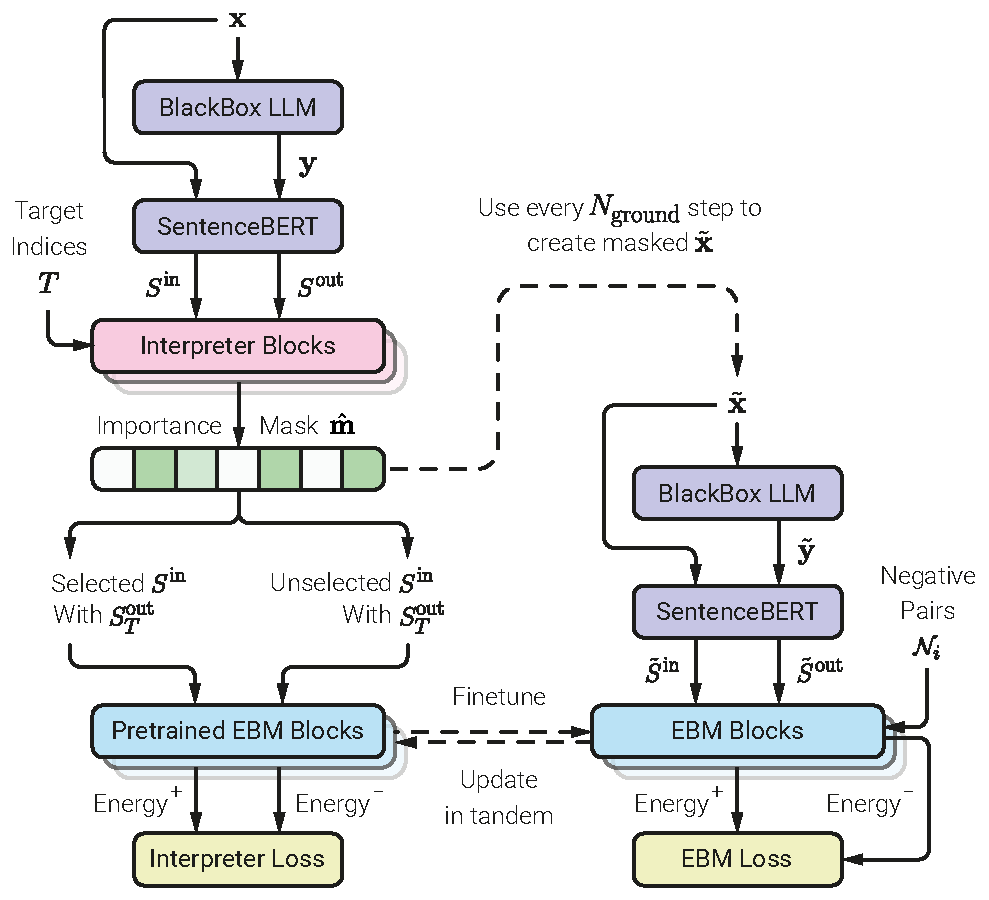
\includegraphics[width=0.76\textwidth]{figures/Fig-Joint-Training-Pipeline-V4.pdf}
    \caption{خط‌لوله‌ی آموزش مشترک شبکه‌های مفسر و انرژی}\label{fig:chap4_pipeline_joint_training}
\end{figure}

در این الگوریتم، پارامترهای مفسر ($\alpha$) و پارامترهای شبکه‌ی انرژی ($\theta$) به‌صورت متناوب و در دو گام مجزا به‌روزرسانی می‌شوند. فرض کنید در گام آموزشی $k$ام قرار داریم و مقادیر پارامترها به‌صورت $\theta^{(k)}$ و $\alpha^{(k)}$ نمادگذاری شده‌اند.

\paragraph{گام اول: به‌روزرسانی مفسر (تقطیر دانش).}
در گام‌های آموزشی متعارف (سمت چپ شکل~\ref{fig:chap4_pipeline_joint_training})، پارامترهای شبکه‌ی انرژی ($\theta^{(k-1)}$) ثابت نگه‌داشته می‌شوند. مفسر، بردار ماسک نرم $\hat{\mathbf{m}}$ را با استفاده از تقریب برنولی (معادله‌ی~\ref{eq:chap4_interp_sigmoid}) تولید می‌کند. سپس پارامترهای آن ($\alpha$) از طریق گرادیان نزولی به‌روزرسانی می‌شوند تا تابع هدف مفسر (معادله‌ی~\ref{eq:chap4_interpreter_loss_final}) را کمینه کنند:
\begin{equation}\label{eq:chap4_update_interpreter}\vspace{0.25cm}
    \begin{split}
        \alpha^{(k)} \leftarrow \alpha^{(k-1)} - \eta_{\alpha} \nabla_\alpha \Big( &\mathcal{E}_{\text{\lr{LM}}}\big(\mathbf{x} \odot \hat{\mathbf{m}}, \mathbf{y}_T; \theta^{(k-1)}\big) \\
        &- \mathcal{E}_{\text{\lr{LM}}}\big(\mathbf{x} \odot (\mathbf{1} - \hat{\mathbf{m}}), \mathbf{y}_T; \theta^{(k-1)}\big) + \lambda_{\text{\lr{sparse}}} \|\hat{\mathbf{m}}\|_1 \Big)
    \end{split}\vspace{0.25cm}
\end{equation}
که در آن $\eta_{\alpha}$ نرخ یادگیری مفسر و $\hat{\mathbf{m}} = \mathcal{IN}(\mathbf{x}, \mathbf{y}, T; \alpha^{(k-1)})$ است. در این گام، مفسر دانش موجود در چشم‌انداز انرژی را برای ارتقای قدرت استخراج پیش‌آیندها تقطیر می‌کند.

\paragraph{گام دوم: تطبیق و لنگراندازی دوره‌ای.}
به‌منظور هم‌تراز نگه‌داشتن \lr{EBM} با توزیع ماسک‌های تولیدشده توسط مفسر، هر $N_{\text{\lr{ground}}}$ گام یک‌بار، فرایند لنگراندازی دوره‌ای\enfootnote{periodic grounding} اجرا می‌شود (سمت راست شکل~\ref{fig:chap4_pipeline_joint_training}). ابتدا ماسک سخت بر پرامپت اعمال می‌شود تا جملات فیلترشده از ورودی حذف شوند (معادله‌ی~\ref{eq:chap4_interp_hard_mask}):
\begin{equation*}
    \mathbf{x}_{\text{\lr{hard}}} = \mathbf{x} \odot \mathbb{I}(\hat{\mathbf{m}} > \epsilon)
\end{equation*}
سپس، این پرامپت از طریق رابط برنامه‌نویسی به مدل جعبه‌سیاه ارسال می‌گردد تا خروجی متناظر آن ثبت شود:
\begin{equation}\label{eq:chap4_query_llm}
    \tilde{\mathbf{y}} = f_\theta(\mathbf{x}_{\text{\lr{hard}}})
\end{equation}
این فرایند یک جفت مشاهداتی جدید $(\mathbf{x}_{\text{\lr{hard}}}, \tilde{\mathbf{y}})$ فراهم می‌سازد که بازتاب‌دهنده‌ی رفتار مدل جعبه‌سیاه در قبال پرامپت تقلیل‌یافته است. در نهایت، پارامترهای شبکه‌ی انرژی ($\theta$) بر روی این داده‌ی جدید با استفاده از تابع زیان دوگانه (معادله‌ی~\ref{eq:chap4_ebm_total_loss}) تنظیم می‌شوند.

در این گام، به دلیل نبود پاسخ انسانی مرجع برای پرامپت مخدوش $\mathbf{x}_{\text{\lr{hard}}}$، مجموعه‌ی منفی وفاداری ($\mathcal{N}^{\text{\lr{fid}}}$) با نمونه‌برداری از سایر مدل‌های پایه بازتعریف می‌شود تا تضاد توزیعی در آموزش \lr{InfoNCE} برقرار بماند. با در نظر داشتن $\tilde{\mathcal{N}}$ به‌عنوان مجموعه‌ی منفی متناظر، رابطه‌ی به‌روزرسانی پارامترهای انرژی به‌صورت زیر خواهد بود:
\begin{equation}\label{eq:chap4_update_ebm}\vspace{0.05cm}
    \theta^{(k)} \leftarrow \theta^{(k-1)} - \eta_{\theta} \nabla_\theta \Big( (1-\lambda)\mathcal{L}_{\text{\lr{fidelity}}}(\mathbf{x}_{\text{\lr{hard}}}, \tilde{\mathbf{y}}, \tilde{\mathcal{N}}) + \lambda\mathcal{L}_{\text{\lr{dep}}}(\mathbf{x}_{\text{\lr{hard}}}, \tilde{\mathbf{y}}) \Big)
\end{equation}

\begin{algorithm}[ht]
\caption{آموزش مشترک شبکه‌های مفسر و انرژی (بهینه‌سازی تناوبی)}\label{alg:chap4_joint_opt}
\begin{algorithmic}[1]
\vspace{0.25cm}
\Require{} پرامپت $\mathbf{x}$، خروجی $\mathbf{y}$، شاخص‌های هدف خروجی $T$، مفسر مقداردهی‌شده $\mathcal{IN}_\alpha$، مدل جانشین پیش‌آموزش‌دیده $\mathcal{E}_\theta$، بازه‌ی لنگراندازی $N_{\text{\lr{ground}}}$، حد آستانه‌ی $\epsilon$
\vspace{0.25cm}
\For{هر گام آموزشی $k$}
    \vspace{0.15cm}
    \State{} \textbf{// گام اول: به‌روزرسانی مفسر}
    \vspace{0.15cm}
    \State{} تولید ماسک نرم پیوسته: $\hat{\mathbf{m}} \leftarrow \text{\lr{Sigmoid}}(\mathcal{IN}(\mathbf{x}, \mathbf{y}, T; \alpha^{(k-1)}))$
    \State{} تفکیک زیرمجموعه‌ها: $\mathbf{x}_S = \mathbf{x} \odot \hat{\mathbf{m}}$ و $\mathbf{x}_{\text{\lr{discard}}} = \mathbf{x} \odot (\mathbf{1} - \hat{\mathbf{m}})$
    \State{} \parbox[t]{0.95\linewidth}{محاسبه‌ی گرادیان و به‌روزرسانی $\alpha^{(k)}$ جهت کمینه‌سازی زیان مفسر (معادله‌ی~\ref{eq:chap4_update_interpreter}) با منتقد ثابت $\mathcal{E}_{\theta^{(k-1)}}$}
    \vspace{0.25cm}
    \State{} \textbf{// گام دوم: لنگراندازی دوره‌ای و تنظیم ظریف \lr{EBM}}
    \vspace{0.15cm}
    \If{$k \pmod{N_{\text{\lr{ground}}}} == 0$}
        \State{} اعمال ماسک سخت: $\mathbf{x}_{\text{\lr{hard}}} \leftarrow \mathbf{x} \odot \mathbb{I}(\hat{\mathbf{m}} > \epsilon)$
        \State{} استعلام از مدل جعبه‌سیاه: $\tilde{\mathbf{y}} \leftarrow f_\theta(\mathbf{x}_{\text{\lr{hard}}})$
        \State{} \parbox[t]{0.9\linewidth}{محاسبه‌ی گرادیان و به‌روزرسانی $\theta^{(k)}$ جهت کمینه‌سازی تابع زیان انرژی (معادله‌ی~\ref{eq:chap4_update_ebm}) برای جفت $(\mathbf{x}_{\text{\lr{hard}}}, \tilde{\mathbf{y}})$}
    \vspace{0.15cm}
    \Else{}
        \State{} انجماد مدل انرژی: $\theta^{(k)} \leftarrow \theta^{(k-1)}$
    \EndIf{}
    \vspace{0.25cm}
\EndFor{}
\end{algorithmic}
\end{algorithm}

این فرایند لنگراندازی (الگوریتم~\ref{alg:chap4_joint_opt})، دارای دو توجیه نظری در ادبیات یادگیری ماشین است که اجرای آن را برای تثبیت مدل تقویت می‌کند. نخست، بر اساس واکاوی تو و همکاران (۲۰۲۰)~\cite{tu2020improving} پیرامون آموزش مشترک شبکه‌های انرژی و استنتاج، در صورت عدم‌انطباق پویای دو شبکه، مدل انرژی ممکن است دچار نواحی کم‌انرژی کاذب گردد؛ چرا که مفسر در فرایند بهینه‌سازی ممکن است ماسک‌هایی را برگزیند که در چشم‌انداز اولیه‌ی مدل منجمد به‌اشتباه دارای انرژی پایینی هستند. استعلام دوره‌ای از مدل هدف، چشم‌انداز انرژی را با مشاهدات متنی واقعی کالیبره کرده و این عدم‌تعادل‌ها را تعدیل می‌سازد.

افزون بر این، ساوینوف و همکاران (۲۰۲۲)~\cite{savinov2022stepunrolled} در معماری \lr{SUNDAE} نشان دادند مدل‌هایی که با ورودی‌های مخدوش سروکار دارند، چنانچه صرفاً بر روی یک توزیع نویز ایستا آموزش ببینند، در مواجهه با توزیع‌های متغیر نویز با افت تعمیم‌پذیری روبه‌رو می‌شوند. در چارچوب \lr{ESCI}، با تکامل پارامترهای مفسر، توزیع ماسک‌های اعمال‌شده نیز تغییر می‌کند. از این رو، لنگراندازی دوره‌ای از نظر ساختاری با مکانیزم باز کردن گام‌به‌گام\enfootnote{step-unrolling} همسویی دارد؛ فرایندی که تضمین می‌نماید مدل انرژی با توزیع پویای ماسک‌های ایجادشده توسط مفسر همگام باقی بماند.

بدین‌ترتیب، چارچوب دوفازی \lr{ESCI} با تلفیق مدل‌سازی انرژی در سطح گزاره و استنتاج مستهلک‌شده در شبکه‌ی مفسر، رویکردی ساختاریافته برای انتساب در سطح جمله در مدل‌های زبانی جعبه‌سیاه فراهم می‌آورد. این متدولوژی با جایگزینی استعلام‌های مکرر و پرهزینه در زمان استنتاج با یک ارزیابی پیش‌رو، و بهره‌گیری از بهینه‌سازی تناوبی و لنگراندازی دوره‌ای جهت تثبیت بازنمایی‌ها در برابر شوک توزیعی، امکان ممیزی عینی مدل‌های تجاری را بدون نیاز به‌دسترسی به وزن‌ها یا گرادیان‌های درونی فراهم می‌سازد. ارزیابی جامع تجربی، سنجش وفاداری و تحلیل کمّی عملکرد این چارچوب در مقایسه با روش‌های خط‌پایه در فصل~\ref{chap:chapter5_experiments} ارائه خواهد شد.
